
%   Hamzeh Khanpour
%   DIS 2026 talk
%   Perspectives for HET physics studies at a muon-hadron collider at CERN

\documentclass[aspectratio=1610,english]{beamer}

\usepackage{babel}
\usepackage[T1]{fontenc}
\usepackage[utf8]{inputenc}
\usepackage{lmodern}
\usepackage{amsmath,amssymb,bm}
\usepackage{booktabs}
\usepackage{graphicx}
\usepackage{array}
\usepackage{ragged2e}
\usepackage{etoolbox}

\usepackage{tikz}
\usepackage{comment}

\usepackage{tikz-feynman}
\tikzfeynmanset{compat=1.1.0}


\usetikzlibrary{calc,positioning,arrows.meta,decorations.pathmorphing,patterns,shapes.geometric}

\usepackage{hyperref}

\usepackage[table]{xcolor}

\makeatletter
\patchcmd{\itemize}{\raggedright}{\justifying}{}{}
\patchcmd{\beamer@enum@}{\raggedright}{\justifying}{}{}
\patchcmd{\@@description}{\raggedright}{\justifying}{}{}
\makeatother

\mode<beamer>{
    \definecolor{links}{HTML}{2A1B81}
    \hypersetup{pdfpagemode=FullScreen,colorlinks,linkcolor=,urlcolor=links}
    \usetheme[parttitle=rightfooter]{AGH}
}

\graphicspath{{./}{/mnt/data/}}

\definecolor{LHRed}{RGB}{170,20,30}
\definecolor{LHBlue}{RGB}{25,60,180}
\definecolor{LHGreen}{RGB}{0,120,60}
\definecolor{LHOrange}{RGB}{210,110,20}
\definecolor{LHPurple}{RGB}{110,60,160}



\newcommand{\LHCmu}{LH$\mu$C}
\newcommand{\placeholdergraphic}[2]{%
\begin{center}
\fbox{\parbox[c][#2][c]{0.86\textwidth}{\centering\vspace{1ex}\textbf{Placeholder for later screenshot}\\[0.6ex]\small #1\vspace{1ex}}}
\end{center}}



\newcommand{\takehome}[1]{%
\begin{alertblock}{Take-home message}
\small #1
\end{alertblock}}



\title[Perspectives for HET physics studies at \LHCmu]{\justifying {\color{red}Updating:}Perspectives for HET physics studies at a muon-hadron collider at CERN}
\author[Hamzeh Khanpour]{Hamzeh Khanpour\\
{\scriptsize \href{(on behalf of HELP4CERN Study Group)}{(on behalf of HELP4CERN Study Group)}}}

\institute[AGH]{Faculty of Physics and Applied Computer Science\\AGH University of Krakow}

\date{{\setlength{\fboxsep}{4pt}\colorbox{cyan!15}{\strut DIS 2026, Bologna, May 7, 2026}}}
 
 
% \textbf{Contact:} \texttt{help-4-cern@cern.ch}
 
 
\begin{document}
 
 
% --------------------------------------------------------------------------
% Slide 1
% --------------------------------------------------------------------------
\begin{frame} 
	
\begin{tikzpicture}[remember picture,overlay]
\node[anchor=north east, xshift=-0.60cm, yshift=-1.50cm]
at (current page.north east)
{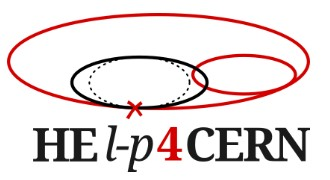
\includegraphics[width=2.5cm]{HELP4CERN.jpg}};
\end{tikzpicture} 

\titlepage 

\end{frame} 




% --------------------------------------------------------------------------
% Slide 2
% --------------------------------------------------------------------------
\begin{frame}{Outline}
	
\tableofcontents
	
\begin{tikzpicture}[remember picture,overlay]
\node[anchor=north east, xshift=-0.60cm, yshift=-1.50cm]
at (current page.north east)
{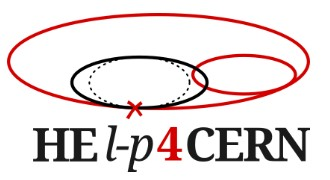
\includegraphics[width=2.5cm]{HELP4CERN.jpg}};
\end{tikzpicture}
	
\end{frame}





\section{LH$\mu$C@CERN: physics motivation and benchmarks}


% --------------------------------------------------------------------------
% Slide 3
% --------------------------------------------------------------------------
\begin{frame}{Why a muon--hadron collider for HET physics?}

\begin{itemize}
\justifying
\item A muon-hadron collider combines the clean lepton-hadron initial state of DIS with a multi-TeV centre-of-mass energy, opening a new regime for Higgs, electroweak, top, and BSM studies.

\item Relative to an electron-proton collider, replacing the electron beam by a muon beam strongly relaxes the synchrotron-radiation limitation, allowing significantly higher beam energies and hence much larger hard-scattering rates, and pushes the centre-of-mass energy deep into the multi-TeV regime.
	
\item Relative to proton-proton collisions, the $\mu p$ environment remains experimentally cleaner, with smaller QCD backgrounds for many precision and BSM channels.
\end{itemize}


\begin{alertblock}{Three complementary physics paths at LH$\mu$C}
\small
\justifying
LH$\mu$C combines three powerful and complementary directions: a strong QCD programme, high-precision Higgs/top/electroweak measurements, and a powerful probe of physics beyond the Standard Model.
\end{alertblock}

\begin{tikzpicture}[remember picture,overlay]
\node[anchor=north east, xshift=-0.10cm, yshift=-1.25cm]
at (current page.north east)
{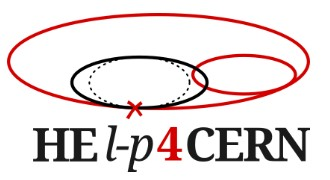
\includegraphics[width=1.5cm]{HELP4CERN.jpg}};
\end{tikzpicture}
\end{frame}



% --------------------------------------------------------------------------
% Slide 4
% --------------------------------------------------------------------------
\begin{frame}{Benchmark working points used in this talk}
	
\begin{columns} 
\begin{column}{0.70\textwidth}
\begin{itemize}
\justifying
\small
\item The present talk focuses on the physics case of the LH$\mu$C, using the current HELP4CERN working benchmarks: 
				
\item The nominal baseline is
\[
E_\mu=500~\mathrm{GeV}, \, E_p=7~\mathrm{TeV},
\, \sqrt{s} \simeq 3.7~\mathrm{TeV},
\]
with a $\mathcal{L}_{\mathrm{int}}=250~\mathrm{fb}^{-1}$.
				
\item The main upgrade scenario is
\[
E_\mu=1~\mathrm{TeV}, \, E_p=7~\mathrm{TeV},
\, \sqrt{s}\simeq 5.3~\mathrm{TeV},
\]
with a $\mathcal{L}_{\mathrm{int}}=1000~\mathrm{fb}^{-1}$.
				
{
\setbeamercolor{block title}{fg=white,bg=green!55!black}
\setbeamercolor{block body}{fg=black,bg=green!10}
	
\begin{block}{LH$\mu$C physics message}
\justifying
\scriptsize
These working points are sufficient to demonstrate the main message of LH$\mu$C: already at the 500~GeV baseline, LH$\mu$C enters the multi-TeV regime and becomes highly competitive for Higgs, top, electroweak, $\gamma\gamma$, and representative BSM studies.
\end{block}
}

\end{itemize}
\end{column}
		
\begin{column}{0.42\textwidth}
\begin{alertblock}{Benchmarks}
\small
\justifying
\begin{tabular}{@{}ll@{}}
\textbf{Machine} & \textbf{Benchmark} \\[0.2em]
LHeC & $E_e=20,\,50$ GeV \\
LH$\mu$C baseline & $E_\mu=500$ GeV \\
LH$\mu$C upgrade & $E_\mu=1$ TeV
\end{tabular}
				
\vspace{0.1em}
				
\begin{tabular}{@{}ll@{}}
\textbf{Configuration} & \textbf{Value} \\[0.2em]
$\sqrt{s}_{\mu p}$ (baseline) & $\simeq 3.7$ TeV \\
$\sqrt{s}_{\mu p}$ (upgrade) & $\simeq 5.3$ TeV \\
$\mathcal{L}_{\rm int}$ (baseline) & $250~\mathrm{fb}^{-1}$ \\
$\mathcal{L}_{\rm int}$ (upgrade) & $1000~\mathrm{fb}^{-1}$
\end{tabular}
\end{alertblock}
			
\centering
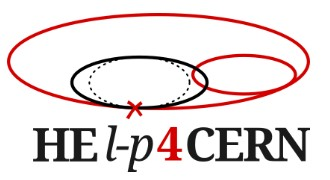
\includegraphics[width=0.5\linewidth]{HELP4CERN.jpg}
{\scriptsize
\setlength{\fboxsep}{4pt}%
\colorbox{blue!20}{\href{https://agenda.infn.it/event/47074/overview}{\strut See talk by Krzysztof Piotrzkowski}}%
}
\end{column}
\end{columns}
\end{frame}



% --------------------------------------------------------------------------
% Slide 5
% --------------------------------------------------------------------------
\begin{frame}{Kinematic reach and QCD physics landscape}

\begin{columns} 
\begin{column}{0.55\textwidth}
\begin{figure}
\centering
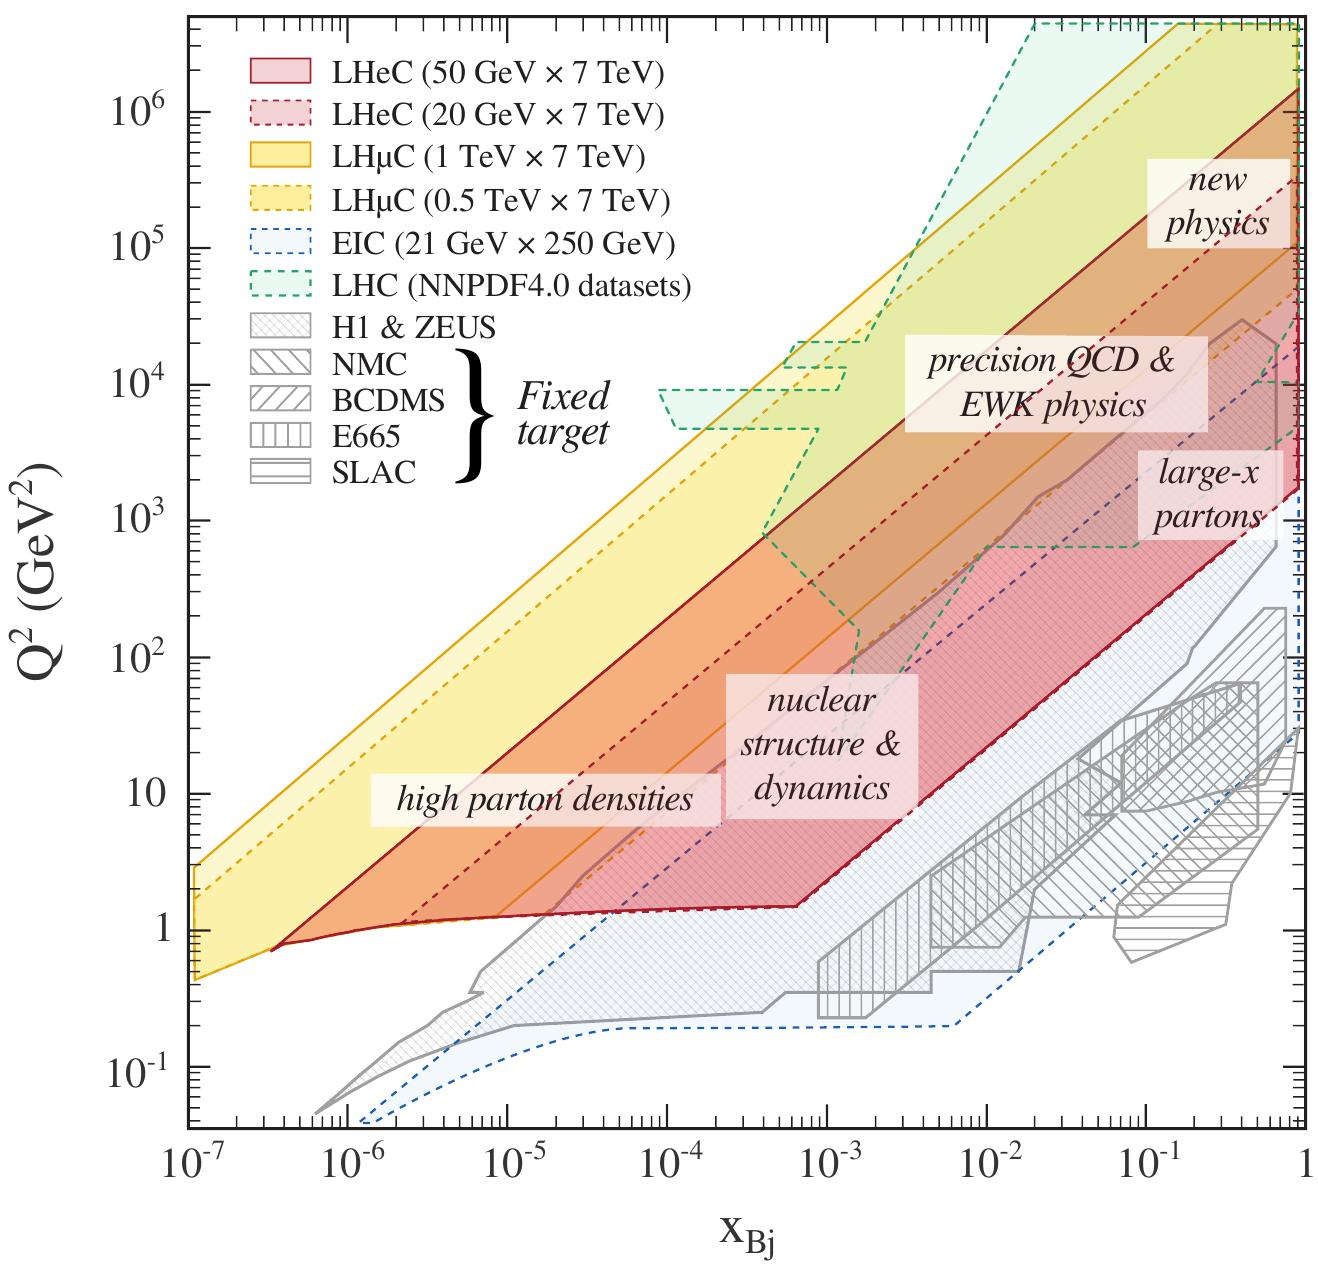
\includegraphics[width=\linewidth]{LHmuC_xQ2.jpg}
\justifying \scriptsize Available $(x,Q^2)$ plane for the proposed LH$\mu$C, compared with fixed-target, collider, and EIC kinematic coverage.
\end{figure}
\end{column}


\begin{column}{0.61\textwidth}
{
\setbeamercolor{block title}{fg=white,bg=blue!45!black}
\setbeamercolor{block body}{fg=black,bg=blue!10}
	
\begin{block}{QCD program at LH$\mu$C}
\begin{itemize}
\justifying
\item The multi-TeV $\mu p$ configuration extends the DIS kinematic coverage well beyond HERA and significantly beyond the LHeC.
\item The same machine that reaches extreme $x$ and $Q^2$ also strengthens the QCD programme through improved access to proton PDFs, and precise determinations of $\alpha_s$. 
\item This motivates the broader CERN bridge-project narrative: LH$\mu$C strengthens both the QCD frontier and the HET/BSM programme.
\end{itemize}
\end{block}
}

\centering
\scriptsize
{\setlength{\fboxsep}{4pt}\colorbox{blue!20}{\href{https://agenda.infn.it/event/47074/overview}{\strut See talk by Piotr Kotko}}}

\end{column}
\end{columns}
\begin{tikzpicture}[remember picture,overlay]
\node[anchor=north east, xshift=-0.10cm, yshift=-1.25cm]
at (current page.north east)
{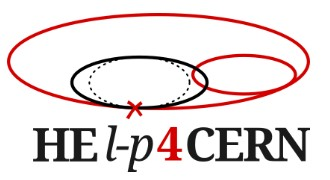
\includegraphics[width=1.5cm]{HELP4CERN.jpg}};
\end{tikzpicture}
\end{frame}





\section{HET overview: Higgs, electroweak and top}



% --------------------------------------------------------------------------
% Slide 6
% --------------------------------------------------------------------------
\begin{frame}{Representative HET benchmark cross sections}
\begin{columns}%[T,onlytextwidth]
		
%---------------------------------------
\begin{column}{0.40\textwidth}	
\begin{block}{What does this table show?}
\small
\justifying LH$\mu$C as a genuine HET factory:
Higgs production is large enough to support precision Higgs physics, including benchmark coupling studies {\color{red}\&} 
the top sector benefits the most, enabling both precision top measurements and sensitivity to rare top processes, {\color{red}\&}  
even the 500~GeV baseline opens a qualitatively new regime for electroweak, EFT, and BSM physics.  
\end{block}
\end{column}



%---------------------------------------
\begin{column}{0.56\textwidth}
			
{
\setbeamercolor{block title}{fg=white,bg=red!65!black}
\setbeamercolor{block body}{fg=black,bg=red!3}
				
\begin{block}{Benchmark inclusive cross sections}
\centering
%\small
\renewcommand{\arraystretch}{1.2}
\resizebox{\linewidth}{!}{%
\begin{tabular}{lcccc}
\toprule
Process & 20 GeV & 50 GeV & 500 GeV & 1 TeV \\
& LHeC & LHeC & LH$\mu$C & LH$\mu$C \\
\midrule
$\sigma(\ell p\to \nu_\ell H+\mathrm{jet}+X)$ [fb]
& 52 & 164 & 438 & 731 \\
					
$\sigma(\ell p\to \ell H+\mathrm{jet}+X)$ [fb]
& 5.6 & 19 & 135 & 221 \\
							
$\sigma(\ell p\to \ell\, t\bar t +X)$ [pb]
& 0.0015 & 0.0323 & 1.03 & 2.23 \\
							
$\sigma(\ell p\to \nu_\ell t +X)$ [pb]
& 0.55 & 2.89 & 21.26 & 36.77 \\
\bottomrule
\end{tabular}%
}
				
%\vspace{0.5em}
%{\tiny \justifying
%Benchmark inclusive cross sections for representative Higgs and top production processes at the LHeC and LH$\mu$C working points.
%}
					
\vspace{0.4em}	
\begin{alertblock}{Key comparisons}
\small
\justifying
Relative to the 50~GeV LHeC benchmark, the 500~GeV LH$\mu$C increases rates by approximately: $\sim 2.7$ for charged-current Higgs production, $\sim 7$ for single-top production, and $\sim 32$ for $t\bar t$ production.
\end{alertblock}
					
\end{block}
}
			
\end{column}
\end{columns}
	
\begin{tikzpicture}[remember picture,overlay]
\node[anchor=north east, xshift=-0.10cm, yshift=-1.25cm]
at (current page.north east)
{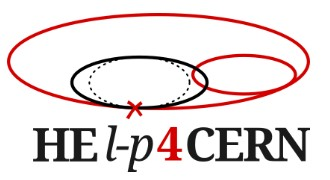
\includegraphics[width=1.5cm]{HELP4CERN.jpg}};
\end{tikzpicture}
	
\end{frame}




\section{Precision Higgs physics at \LHCmu} 


% --------------------------------------------------------------------------
% Slide 7
% --------------------------------------------------------------------------
\begin{frame}{Higgs production at \LHCmu: channels, rates, and statistics}
	
\begin{columns}%[T,onlytextwidth]
		
%========================================
% Left column: text
%========================================
\begin{column}{0.65\textwidth}
\begin{itemize}
\justifying
\small
\item Higgs production is dominated by CC VBF, with a subleading but still sizeable NC contribution.
				
\item Using the current benchmarks:
\begin{itemize}
\justifying
\small
\item 500~GeV \LHCmu: $\sigma_{\mathrm{CC}}\simeq 438$~fb, $\sigma_{\mathrm{NC}}\simeq 135$~fb,
\item 1~TeV \LHCmu: $\sigma_{\mathrm{CC}}\simeq 731$~fb, $\sigma_{\mathrm{NC}}\simeq 221$~fb.
\end{itemize}
				
\item For the benchmark integrated luminosities, these correspond to roughly:
\begin{itemize}
\justifying
\small
\item $1.10\times10^5$ CC Higgs and $3.38\times10^4$ NC Higgs events at 500~GeV,
\item $7.31\times10^5$ CC Higgs and $2.21\times10^5$ NC Higgs events at 1~TeV.
\end{itemize}
				
\item This already motivates precision Higgs-coupling studies beyond a mere rescaling of LHeC expectations.
\end{itemize}
\end{column}
		
%========================================
% Right column: diagrams + plot
%========================================
\begin{column}{0.45\textwidth}
			
%----------------------------------------
% Small diagrams on top
%----------------------------------------
\begin{columns}[T,onlytextwidth]
				
%----------------------
% CC diagram
%----------------------
\begin{column}{0.45\textwidth}
\centering
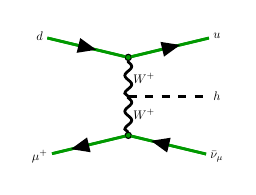
\begin{tikzpicture}[scale=0.45, transform shape]
\begin{feynman}
\vertex (i1) at (-2.5,  1.7) {\(d\)};
\vertex (i2) at (-2.5, -1.7) {\(\mu^{+}\)};
\vertex [dot, fill=green!60!black, minimum size=5pt] (v1) at (0,1.1) {};
\vertex [dot, fill=green!60!black, minimum size=5pt] (v2) at (0,-1.1) {};
\vertex (o1) at (2.5,  1.7) {\(u\)};
\vertex (o2) at (2.5, -1.7) {\(\bar{\nu}_{\mu}\)};
\vertex (h1) at (2.5,0.0) {\(h\)};
\vertex (m1) at (0,0.0);
							
\diagram*{
(i1) -- [fermion, draw=green!60!black, line width=1.0pt] (v1)
-- [fermion, draw=green!60!black, line width=1.0pt] (o1),
(i2) -- [anti fermion, draw=green!60!black, line width=1.0pt] (v2)
-- [anti fermion, draw=green!60!black, line width=1.0pt] (o2),
(v1) -- [boson, edge label=\(W^{+}\), line width=1.0pt] (m1),
(m1) -- [boson, edge label=\(W^{+}\), line width=1.0pt] (v2),
(m1) -- [scalar, line width=1.0pt] (h1),
};
\end{feynman}
\end{tikzpicture}
					
\vspace{0.05em}
{\scriptsize CC: \(\mu^{+} p \to \bar{\nu}_{\mu}\,j\,h\)}
\end{column}
				
%----------------------
% NC diagram
%----------------------
\begin{column}{0.45\textwidth}
\centering
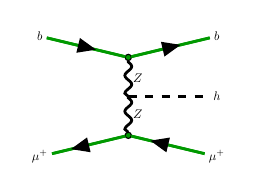
\begin{tikzpicture}[scale=0.45, transform shape]
\begin{feynman}
\vertex (i1) at (-2.5,  1.7) {\(b\)};
\vertex (i2) at (-2.5, -1.7) {\(\mu^{+}\)};
\vertex [dot, fill=green!60!black, minimum size=5pt] (v1) at (0,1.1) {};
\vertex [dot, fill=green!60!black, minimum size=5pt] (v2) at (0,-1.1) {};
\vertex (o1) at (2.5,  1.7) {\(b\)};
\vertex (o2) at (2.5, -1.7) {\(\mu^{+}\)};
\vertex (h1) at (2.5,0.0) {\(h\)};
\vertex (m1) at (0,0.0);
							
\diagram*{
(i1) -- [fermion, draw=green!60!black, line width=1.0pt] (v1)
-- [fermion, draw=green!60!black, line width=1.0pt] (o1),
(i2) -- [anti fermion, draw=green!60!black, line width=1.0pt] (v2)
-- [anti fermion, draw=green!60!black, line width=1.0pt] (o2),
(v1) -- [boson, edge label=\(Z\), line width=1.0pt] (m1),
(m1) -- [boson, edge label=\(Z\), line width=1.0pt] (v2),
(m1) -- [scalar, line width=1.0pt] (h1),
};
\end{feynman}
\end{tikzpicture}
					
\vspace{0.05em}
{\scriptsize NC: \(\mu^{+} p \to \mu^{+}\,j\,h\)}
\end{column}
				
\end{columns}
			
\vspace{0.20em}
			
%----------------------------------------
% Cross-section plot
%----------------------------------------
\centering
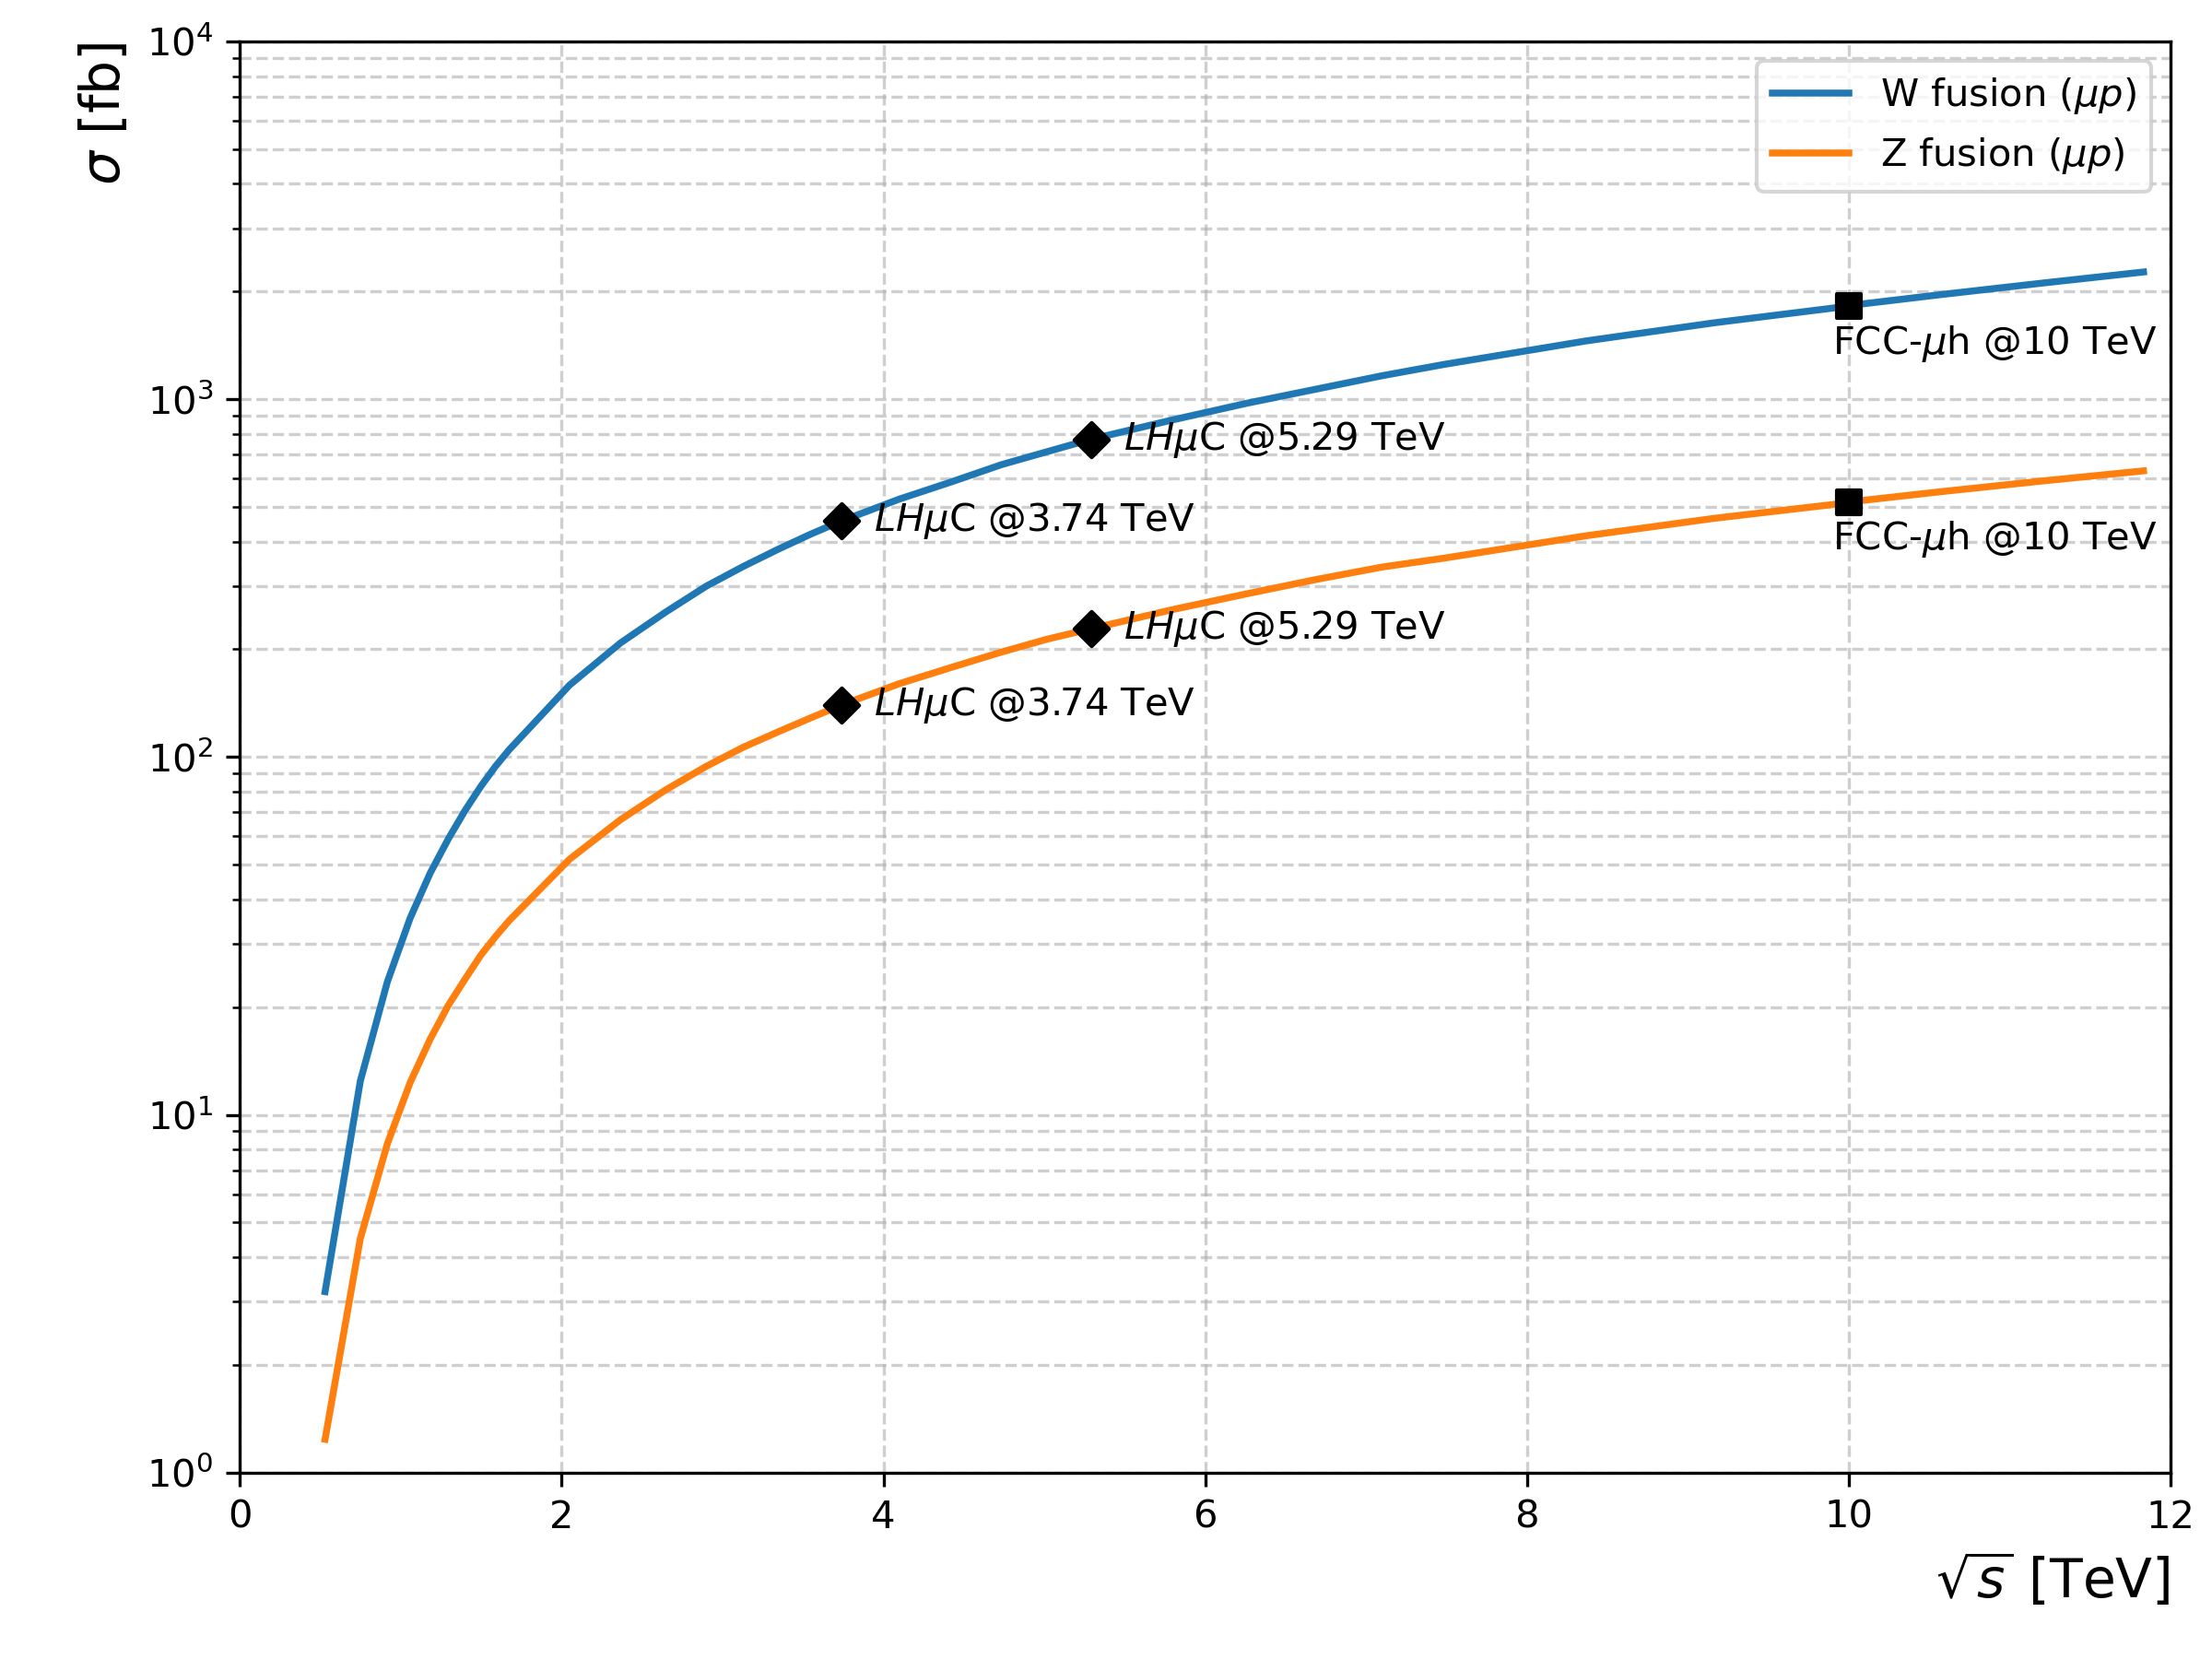
\includegraphics[width=0.99\linewidth]{mupVBFH_xsec_nocut.png}
%\vspace{0.35em}			
\justifying \scriptsize Higgs boson production cross sections at LH$\mu$C for the CC (\(W\)-fusion) and subleading NC (\(Z\)-fusion) contributions.
		
\end{column}
		
\end{columns}
	
%----------------------------------------
% HELP4CERN logo
%----------------------------------------
\begin{tikzpicture}[remember picture,overlay]
\node[anchor=north east, xshift=-0.10cm, yshift=-1.25cm]
at (current page.north east)
{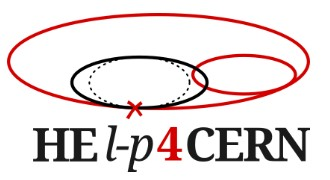
\includegraphics[width=1.5cm]{HELP4CERN.jpg}};
\end{tikzpicture}
	
\end{frame}





% --------------------------------------------------------------------------
% Slide 8
% --------------------------------------------------------------------------
\begin{frame}{Precision Higgs case study: $h\to b\bar b$ and coupling prospects}
	
\begin{columns}[T]

%----------------------------------------
\begin{column}{0.65\textwidth}
\begin{itemize}
\justifying
\small
				
\item A concrete benchmark study already exists for the charged-current VBF channel
\[
p\mu^{+}\to j\,\bar{\nu}_{\mu}\,h,\qquad h\to b\bar b .
\]
				
\item Analysis chain used in this study:
\begin{itemize}
\justifying
\small
\item MG5\_aMC@NLO + Pythia6 + FastJet + Delphes,
\item LHeC-like asymmetric detector setup and 75\% $b$-tagging efficiency,
\item selection with exactly two $b$-jets and
\[
|m_{bb}-m_h|<25~\mathrm{GeV}.
\]
\end{itemize}
				
\item This gives a benchmark on the measurable rate which can be translated into a sensitivity on $g_{hbb}$:
\[
\sigma(p\mu^{+}\to j\,\bar{\nu}_{\mu}\,b\bar b)
\;\propto\;
\frac{g_{hWW}^2\,g_{hbb}^2}{\Gamma_h},
\]

				
\end{itemize}
\end{column}
		
		
		
%----------------------------------------
\begin{column}{0.45\textwidth}
\centering
\scriptsize
\renewcommand{\arraystretch}{1.15}
\setlength{\tabcolsep}{4pt}
\begin{tabular}{lcc}
\toprule
& LH$\mu$C-500 & LH$\mu$C-1000 \\
\midrule
$\sigma_{\rm sig}$ [pb]      & 0.24 & 0.39 \\
$\sigma_{\rm bgd\text{-}Z}$ [pb] & 0.30 & 0.50 \\
$\sigma_{\rm bgd\text{-}mj}$ [pb] & 357.9 & 563.8 \\
\midrule
$\Delta \sigma/\sigma$ & 1.19\% & 0.69\% \\
$\Delta g_{hbb}/g_{hbb}$ & 0.77\% & 0.60\% \\
\bottomrule
\end{tabular}

\justifying
\vspace{0.35em}			
{\scriptsize
Benchmark charged-current $h\to b\bar b$ sensitivities in our study.
The quoted coupling reach follows from the benchmark rate measurement after propagating the external uncertainty on $g_{hWW}^2/\Gamma_h$.
}
\vspace{0.2em}
\begin{alertblock}{Key finding}
\scriptsize
\justifying
The current \LHCmu benchmark study already reaches sub-percent sensitivity to
$g_{hbb}$ in the charged-current Higgs channel, turning the large production rates into
a concrete precision-Higgs case.
\end{alertblock}

\end{column}
\end{columns}

\begin{tikzpicture}[remember picture,overlay]
\node[anchor=north east, xshift=-0.10cm, yshift=-1.25cm]
at (current page.north east)
{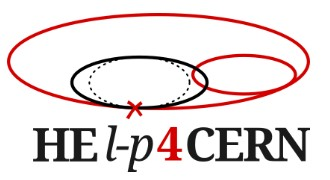
\includegraphics[width=1.5cm]{HELP4CERN.jpg}};
\end{tikzpicture}
	
\end{frame}







% --------------------------------------------------------------------------
% Slide 9
% --------------------------------------------------------------------------
\begin{frame}{Broader Higgs-coupling reach: a global-fit picture}
	
\begin{columns}[T]
		
%----------------------------------------
\begin{column}{0.60\textwidth}
\begin{itemize}
\justifying 
\small 
\item Beyond the dedicated $h\to b\bar b$ benchmark, we also
examined a Higgs coupling fit in the kappa-3 framework.

\item These results are obtained in a first explorative study:
\begin{itemize}
\justifying 
\scriptsize 
\item the same systematic factors as in the underlying LHeC-based setup,
\item the statistical error is rescaled using the benchmark LH$\mu$C cross sections,
\item and the fit results shown here were obtained with the \textsc{SMEFiT} framework.
\end{itemize}
				
\item The strongest visible improvement is in the vector sector:
{\scriptsize
\[
\delta\kappa_W \simeq 0.29\% \;\;(\mathrm{LH}\mu\mathrm{C}\text{-}0.5\mathrm{TeV}),\,
0.19\% \;\;(\mathrm{LH}\mu\mathrm{C}\text{-}1\mathrm{TeV}).
\]
}				
\item The clearest message of the current exploratory fit is the strong projected improvement in the vector sector, especially for \(\kappa_W\) and \(\kappa_Z\), at the higher-energy \LHCmu stages.

\end{itemize}
\end{column}

%----------------------------------------
\begin{column}{0.50\textwidth}
\vspace{0.9em}
\centering
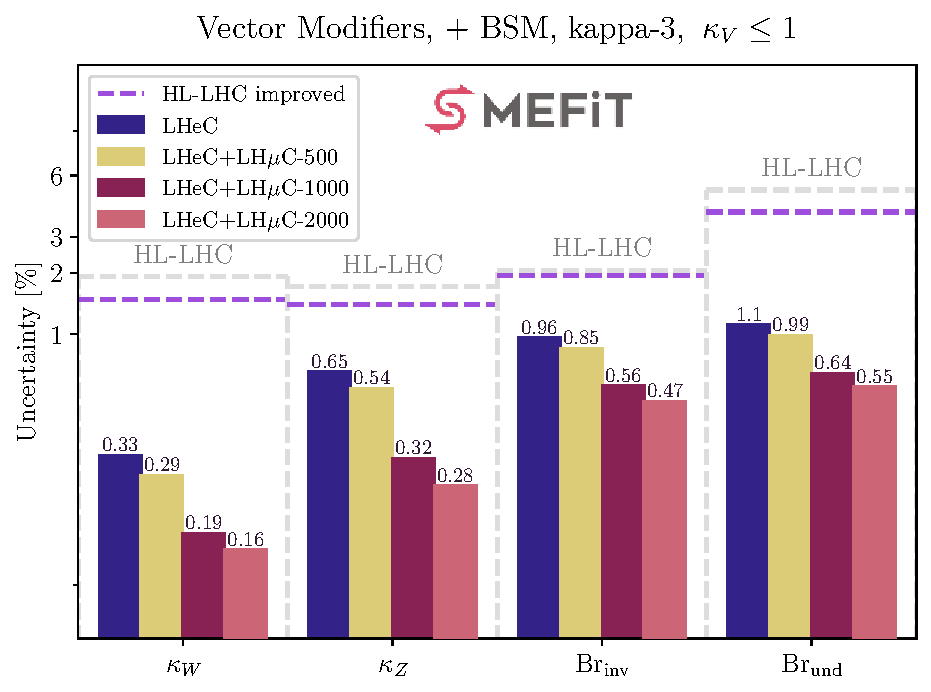
\includegraphics[width=\linewidth]{LHmuC_vector.pdf}
\vspace{0.2em}
\justifying \scriptsize Exploratory vector-modifier result in the kappa-3 framework. The panel compares HL-LHC-based benchmarks with LHeC and with LHeC+LH$\mu$C stages.
\end{column}

\end{columns}

\begin{tikzpicture}[remember picture,overlay]
\node[anchor=north east, xshift=-0.10cm, yshift=-1.25cm]
at (current page.north east)
{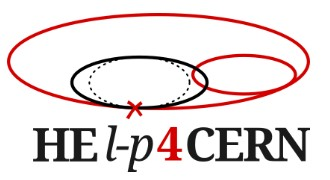
\includegraphics[width=1.5cm]{HELP4CERN.jpg}};
\end{tikzpicture}
	
\end{frame}






% --------------------------------------------------------------------------
% Slide 10
% --------------------------------------------------------------------------
% --------------------------------------------------------------------------
% Electroweak programme and EFT opportunities
% --------------------------------------------------------------------------
\begin{frame}{Electroweak programme and EFT opportunities}
	
\begin{columns}[T]%[T,onlytextwidth]
		
%========================================
% Left alert box
%========================================
\begin{column}{0.48\textwidth}
\begin{alertblock}{EW precision reach at LH$\mu$C}
\justifying
\small
\begin{itemize}
\justifying
\item Beyond Higgs rates, LH$\mu$C offers a broader electroweak programme based on high-$Q^2$ DIS, vector-boson fusion, and photon-induced reactions.
					
\item The larger kinematic span relative to the LHeC is expected to strengthen sensitivity to key electroweak observables, in particular $m_W$ and $\sin^2\theta_W$, while also extending the SMEFT lever arm.
					
\item Overall, LH$\mu$C is expected to extend the precision electroweak reach beyond that projected for the LHeC.
\end{itemize}
\end{alertblock}
			
\end{column}
		
%========================================
% Right alert box
%========================================
\begin{column}{0.58\textwidth}
\begin{alertblock}{Highlighted EW / EFT opportunities}
\justifying
\small
\begin{itemize}
\justifying
\item High-scale measurements of the weak mixing angle and its running,
					
\item Precision light-quark weak neutral-current couplings via $\gamma Z$ interference and $Z$ exchange,
					
\item Improved sensitivity to $m_W$ in a clean DIS environment,
					
\item Electroweak/top measurements linked to the $Wtb$ vertex and direct sensitivity to $V_{ts}$,
					
\item SMEFT directions complementary to those probed at $pp$ and $e^+e^-$ machines,
					
\item Photon-induced EFT sensitivity in $\gamma\gamma\to W^+W^-$, $ZZ$, and heavy final states.
\end{itemize}
\end{alertblock}
			
\end{column}
		
\end{columns}
	
\begin{tikzpicture}[remember picture,overlay]
\node[anchor=north east, xshift=-0.10cm, yshift=-1.25cm]
at (current page.north east)
{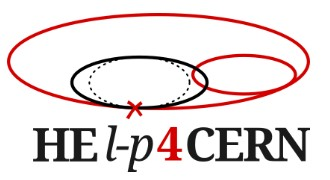
\includegraphics[width=1.5cm]{HELP4CERN.jpg}};
\end{tikzpicture}
	
\end{frame}




\section{High-energy $\gamma\gamma$ physics at \LHCmu}



% --------------------------------------------------------------------------
% Slide 11
% --------------------------------------------------------------------------
\begin{frame}{High-energy $\gamma \gamma$ physics is a natural part of the \LHCmu{} programme}
\begin{columns}[T]
\begin{column}{0.55\textwidth}

\begin{alertblock}{Interesting HET directions}
\begin{itemize}
\justifying
\small
\item \LHCmu{} naturally operates as {\textit {a high-energy $\gamma\gamma$ collider}}.% through photons radiated from the incoming muon and proton beams.
\item In the 500 GeV baseline, the effective $\gamma\gamma$ centre-of-mass energy extends into the multi-TeV regime, opening a broad programme of clean exclusive measurements.
\justifying
\footnotesize
\setlength{\itemsep}{0.1em}
\begin{itemize}
\item anomalous $\tau$ moments,
\item $\gamma\gamma\to W^+W^-$ and anomalous quartic gauge couplings (qQGC),
\item loop-induced $\gamma\gamma\to ZZ$,
\item exclusive $t\bar t$ production,
\item light-by-light scattering (LbL) 
\item BSM charged-particle pair production.
\end{itemize}
\end{itemize}
\end{alertblock}

\end{column}


\begin{column}{0.45\textwidth}
\vspace{-0.5cm}
\begin{figure}
\centering
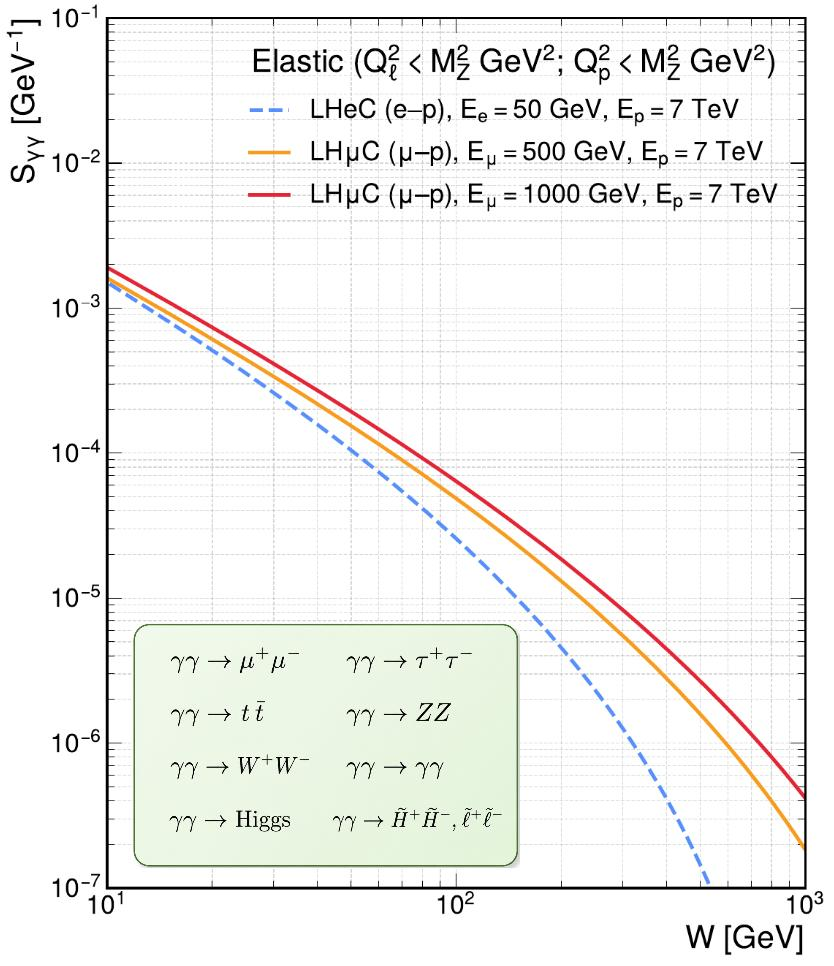
\includegraphics[width=\linewidth]{Sgg_New.jpg}
\justifying \scriptsize Elastic photon-photon luminosity spectrum $S_{\gamma\gamma}$ as a function of the $\gamma\gamma$ invariant mass $W$, comparing the LHeC and  \LHCmu{} benchmark configurations. 
\end{figure}
\end{column}

\end{columns}

\begin{tikzpicture}[remember picture,overlay]
\node[anchor=north east, xshift=-0.10cm, yshift=-1.25cm]
at (current page.north east)
{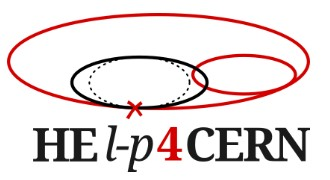
\includegraphics[width=1.5cm]{HELP4CERN.jpg}};
\end{tikzpicture}
\end{frame}






% --------------------------------------------------------------------------
% Slide 12
% --------------------------------------------------------------------------
\begin{frame}{Flagship $\gamma\gamma$ channel: $\tau^+\tau^-$ and anomalous $\tau$ moments}
	
\begin{columns}[T]%[T,onlytextwidth]
		
%========================================
% Left column: text + topology
%========================================
\begin{column}{0.55\textwidth}
	
{
\setbeamercolor{uppercol}{fg=white,bg=green!60!black}
\setbeamercolor{lowercol}{fg=black,bg=green!8}
		
\begin{beamerboxesrounded}[upper=uppercol,lower=lowercol,shadow=true]{LH$\mu$C $\tau^+\tau^-$ physics message}
\justifying
\small
			
\begin{itemize}
\setlength{\itemsep}{0.35em}
\justifying
\item The elastic \(\gamma\gamma\to\tau^+\tau^-\) rate at \LHCmu{}  for $W_0=10$ GeV is already very large, with \(\sigma_{\mathrm{el}}\simeq 58.5\) pb at 3.7 TeV and about \(70.3\) pb at the 5.3 TeV upgrade benchmark. 
\item This provides a high-statistics probe of the \(\gamma\tau\tau\) vertex and anomalous magnetic ($a_\tau$) and electric ($d_\tau$) dipole moments.
\item Anomalous contributions harden the high-\(M_{\tau\tau}\) tail, making the invariant-mass spectrum the key discriminating observable.
\item This is one of the cleanest examples of how \LHCmu{} combines high energy with a low-background exclusive topology.
\end{itemize}
			
\end{beamerboxesrounded}
}
	
\end{column}
		
%========================================
% Right column: figure
%========================================
\begin{column}{0.45\textwidth}
\vspace{-0.5cm}
\begin{figure}
\centering
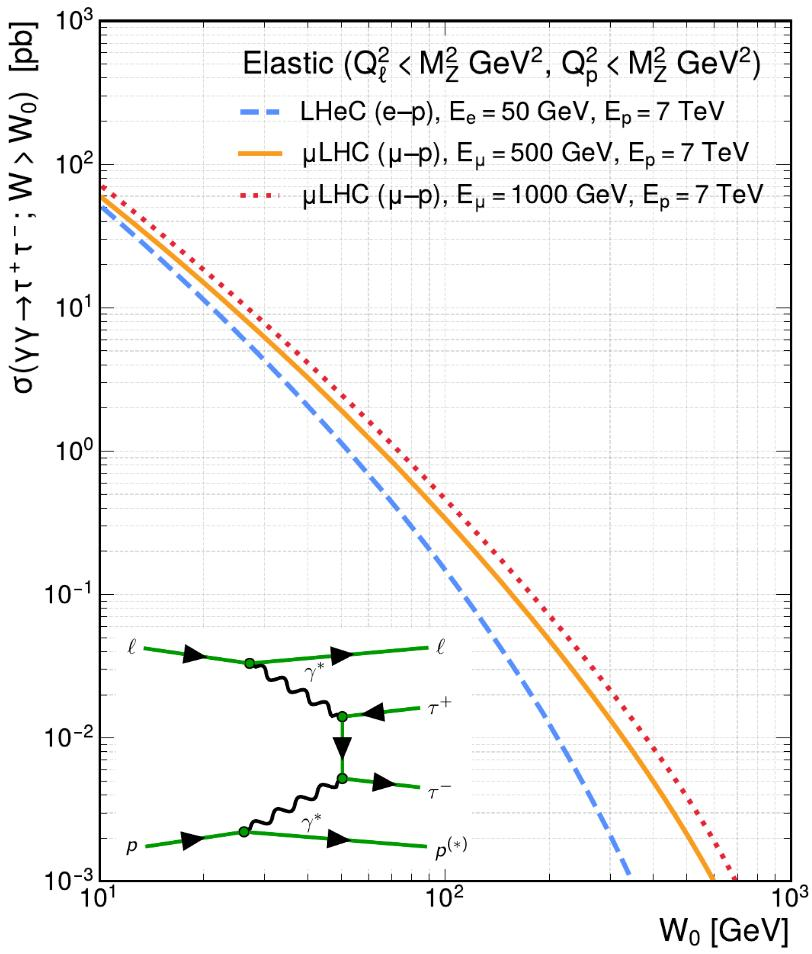
\includegraphics[width=\linewidth,height=0.73\textheight,keepaspectratio]{yytautau.jpg}
\justifying\scriptsize Elastic $\gamma\gamma\to\tau^+\tau^-$ cross section above the threshold $W_0$, comparing the LHeC and \LHCmu{} benchmark configurations.
\end{figure}
\end{column}
		
\end{columns}
	
\begin{tikzpicture}[remember picture,overlay]
\node[anchor=north east, xshift=-0.10cm, yshift=-1.25cm]
at (current page.north east)
{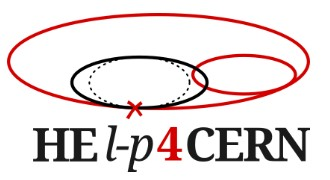
\includegraphics[width=1.5cm]{HELP4CERN.jpg}};
\end{tikzpicture}
	
\end{frame}




% --------------------------------------------------------------------------
% Slide 13
% --------------------------------------------------------------------------

% --------------------------------------------------------------------------
% Merged gamma-gamma summary slide
% --------------------------------------------------------------------------
\begin{frame}{Exclusive $\gamma\gamma$ channels: electroweak, top, and BSM reach}
	
\centering
%	\vspace{-0.35em}
	
\begin{tikzpicture}[x=1cm,y=1cm]
		
%------------------------------------------------
% Styles
%------------------------------------------------
		\tikzset{
			connector/.style={
				draw=blue!65!black,
				line width=1.0pt
			},
			hubbox/.style={
				rounded corners=6pt,
				draw=blue!65!black,
				line width=1.1pt,
				fill=white,
				minimum width=2.9cm,
				minimum height=2.0cm,
				inner sep=3pt,
				align=center
			},
			boxww/.style={
				rounded corners=9pt,
				draw=green!50!black,
				line width=1.15pt,
				fill=green!10,
				minimum width=3.85cm,
				minimum height=2.75cm,
				text width=3.20cm,
				align=center,
				inner sep=4pt
			},
			boxzz/.style={
				rounded corners=9pt,
				draw=violet!55!black,
				line width=1.15pt,
				fill=violet!10,
				minimum width=3.85cm,
				minimum height=2.75cm,
				text width=3.20cm,
				align=center,
				inner sep=4pt
			},
			boxtt/.style={
				rounded corners=9pt,
				draw=orange!70!black,
				line width=1.15pt,
				fill=orange!12,
				minimum width=3.85cm,
				minimum height=2.75cm,
				text width=3.20cm,
				align=center,
				inner sep=4pt
			},
			boxbsm/.style={
				rounded corners=9pt,
				draw=red!65!black,
				line width=1.15pt,
				fill=red!10,
				minimum width=3.85cm,
				minimum height=2.75cm,
				text width=3.20cm,
				align=center,
				inner sep=4pt
			},
			takehome/.style={
				rounded corners=5pt,
				draw=red!60!black,
				line width=0.95pt,
				fill=red!8,
				text width=11.1cm,
				minimum height=0.82cm,
				align=center,
				inner sep=3.5pt
			}
		}
		
%------------------------------------------------
% Central hub
%------------------------------------------------
\node[hubbox] (hub) at (0,0.00) {%
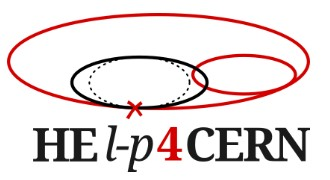
\includegraphics[width=2.05cm]{HELP4CERN.jpg}\\[-0.15em]
{\scriptsize \textbf{Exclusive high-energy}}\\[-0.05em]
{\scriptsize \textbf{$\gamma\gamma$ programme}}
};
		
		%------------------------------------------------
		% Outer nodes
		%------------------------------------------------
		\node[boxww] (ww) at (-4.15,1.65) {%
			{\bfseries \small $\gamma\gamma\to W^+W^-$}\\[0.20em]
%			{\footnotesize largest EW benchmark;}\\
			{\footnotesize Strong aQGC sensitivity comes from}\\
			{\footnotesize the high-$M_{WW}$ tail}\\[0.15em]
%			{\footnotesize $\sigma_{\rm el}\simeq 0.166$ pb at 3.7 TeV}
		};
		
		\node[boxzz] (zz) at (4.15,1.65) {%
			{\bfseries \small $\gamma\gamma\to ZZ$}\\[0.20em]
			{\footnotesize Loop-induced in the SM;}\\
			{\footnotesize clean probe of high-mass}\\
			{\footnotesize electroweak dynamics}\\[0.15em]
%			{\footnotesize $\sigma_{\rm el}\simeq 0.284$ fb at 3.7 TeV}
		};
		
		\node[boxtt] (tt) at (-4.15,-1.85) {%
			{\bfseries \small $\gamma\gamma\to t\bar t$}\\[0.20em]
			{\footnotesize Probes heavy thresholds}\\
			{\footnotesize and top-sector dynamics}\\
			{\footnotesize in exclusive topology}\\[0.15em]
%			{\footnotesize $\sigma_{\rm el}\simeq 0.486$ fb at 3.7 TeV}
		};
		
		\node[boxbsm] (bsm) at (4.15,-1.85) {%
			{\bfseries \small Exclusive BSM pairs}\\[0.20em]
%			{\footnotesize same framework extends to}\\
			{\footnotesize Charged states such as}\\
			{\footnotesize higgsinos and sleptons}\\[0.15em]
%			{\footnotesize qualitative opportunity; no rate quoted here}
		};
		
		%------------------------------------------------
		% Connectors
		%------------------------------------------------
		\draw[connector] (hub.north west) .. controls (-1.1,0.95) and (-2.4,1.35) .. (ww.east);
		\draw[connector] (hub.north east) .. controls ( 1.1,0.95) and ( 2.4,1.35) .. (zz.west);
		\draw[connector] (hub.south west) .. controls (-1.1,-0.85) and (-2.4,-1.35) .. (tt.east);
		\draw[connector] (hub.south east) .. controls ( 1.1,-0.85) and ( 2.4,-1.35) .. (bsm.west);
		
%------------------------------------------------
% Take-home message
%------------------------------------------------
\node[takehome] at (0,-4.00) {%
{\justifying\scriptsize Beyond $\tau^+\tau^-$, the high-energy $\gamma\gamma$ programme at LH$\mu$C spans
electroweak, top, and BSM-sensitive channels in a clean exclusive environment.}
};
		
\end{tikzpicture}
	
\end{frame}
% --------------------------------------------------------------------------






\section{Top physics at \LHCmu{}}






% --------------------------------------------------------------------------
% Slide 14 
% --------------------------------------------------------------------------


% --------------------------------------------------------------------------
% Merged top-physics slide
% --------------------------------------------------------------------------
\begin{frame}{Top physics at \LHCmu{}: production mechanisms and experimental promise}

\begin{columns}[T]%[T,onlytextwidth]

%================================================
% Left column: text
%================================================

\begin{column}{0.65\textwidth}
\small
\begin{itemize} \itemsep 0.45em
\justifying

\item The top sector is one of the clearest HET advantages of \LHCmu{} relative to the LHeC.

\item \textbf{Single-top production} is dominated by charged-current DIS, with representative subprocess $\mu^{+} b \to \bar{\nu}_{\mu}\, t ,$ 
mediated by \(t\)-channel \(W^{+}\) exchange in the 5-flavor scheme.

\item \textbf{Top-pair production} is dominated by neutral-current lepton--gluon scattering, with representative process $\mu^{+} g \to \mu^{+} t\bar t ,$
driven mainly by \(\gamma^\ast g \to t\bar t\), while \(Z^\ast g \to t\bar t\) is subleading.

\item The top advantage is not only a formal cross-section enhancement: it is also supported by favourable acceptance, making the programme experimentally promising after realistic selections.

\end{itemize}
\end{column}


%================================================
% Right column: diagrams
%================================================
\vspace{-0.5em}
\begin{column}{0.47\textwidth}
\vspace{-0.5em}

\centering

%-----------------------------
% Diagram A: single top
%-----------------------------
\begin{minipage}{\linewidth}
\centering
\begin{center}
	\setlength{\fboxsep}{3pt}
	\fcolorbox{black!40}{yellow!20}{%
		\parbox{0.65\linewidth}{\centering\scriptsize\textbf{LO CC single-top production}}%
	}
\end{center}
\vspace{-0.25em}

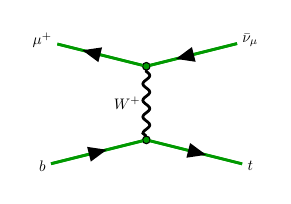
\begin{tikzpicture}[scale=0.55, transform shape]
\begin{feynman}
						\vertex (muin)  at (-2.4,  1.45) {\(\mu^{+}\)};
						\vertex (bin)   at (-2.4, -1.45) {\(b\)};
						\vertex (nuout) at ( 2.4,  1.45) {\(\bar{\nu}_{\mu}\)};
						\vertex (tout)  at ( 2.4, -1.45) {\(t\)};
						
						\vertex [dot, fill=green!60!black, minimum size=5pt] (v1) at (0,  0.85) {};
						\vertex [dot, fill=green!60!black, minimum size=5pt] (v2) at (0, -0.85) {};
						
						\diagram*{
							(muin)  -- [anti fermion, draw=green!60!black, line width=1.0pt] (v1)
							-- [anti fermion, draw=green!60!black, line width=1.0pt] (nuout),
							
							(bin)   -- [fermion, draw=green!60!black, line width=1.0pt] (v2)
							-- [fermion, draw=green!60!black, line width=1.0pt] (tout),
							
							(v1)    -- [boson, edge label'=\(W^{+}\), line width=1.0pt] (v2),
};
\end{feynman}
\end{tikzpicture}

\vspace{0.1em}

\justifying \scriptsize CC DIS with \(t\)-channel \(W^{+}\) exchange (5F scheme) with inclusive rates: \(\sigma=21.26~\mathrm{pb}\), and \(36.77~\mathrm{pb}\). 
\end{minipage}

\vspace{0.2em}

%-----------------------------
% Diagram B: top pair
%-----------------------------
\begin{minipage}{\linewidth}
\centering
\begin{center}
\setlength{\fboxsep}{3pt}
\fcolorbox{black!40}{yellow!20}{%
\parbox{0.65\linewidth}{\centering\scriptsize\textbf{LO NC top-pair production}}%
}
\end{center}
\vspace{-0.25em}

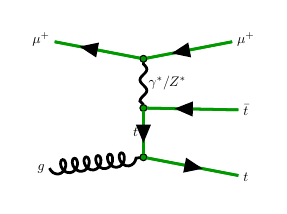
\begin{tikzpicture}[scale=0.50, transform shape]
\begin{feynman}
						\vertex (muin)   at (-2.6,  1.55) {\(\mu^{+}\)};
						\vertex (muout)  at ( 2.6,  1.55) {\(\mu^{+}\)};
						\vertex (gin)    at (-2.6, -1.75) {\(g\)};
						\vertex (tbarout)at ( 2.6, -0.25) {\(\bar t\)};
						\vertex (tout)   at ( 2.6, -1.95) {\(t\)};
						
						\vertex [dot, fill=green!60!black, minimum size=5pt] (v1) at (0,  1.05) {};
						\vertex [dot, fill=green!60!black, minimum size=5pt] (v2) at (0, -0.20) {};
						\vertex [dot, fill=green!60!black, minimum size=5pt] (v3) at (0, -1.45) {};
						
						\diagram*{
							(muin)  -- [anti fermion, draw=green!60!black, line width=1.0pt] (v1)
							-- [anti fermion, draw=green!60!black, line width=1.0pt] (muout),
							
							(v1)    -- [boson, edge label=\(\gamma^{\ast}/Z^{\ast}\), line width=1.0pt] (v2),
							
							(v2)    -- [anti fermion, draw=green!60!black, line width=1.0pt] (tbarout),
							(v2)    -- [fermion, draw=green!60!black, edge label'=\(t\), line width=1.0pt] (v3),
							
							(gin)   -- [gluon, line width=1.0pt] (v3),
							(v3)    -- [fermion, draw=green!60!black, line width=1.0pt] (tout),
						};
\end{feynman}
\end{tikzpicture}

\vspace{0.1em}

\justifying \scriptsize Dominant hard subprocess: \(\gamma^\ast g \to t\bar t\); \(Z^\ast g \to t\bar t\) is subleading with inclusive rates:
\(\sigma=1.03~\mathrm{pb}\), and \(2.23~\mathrm{pb}\). 
\end{minipage}

\end{column}
\end{columns}

%------------------------------------------------
% HELP4CERN logo overlay
%------------------------------------------------
\begin{tikzpicture}[remember picture,overlay]
\node[anchor=north east, xshift=-0.10cm, yshift=-1.25cm]
at (current page.north east)
{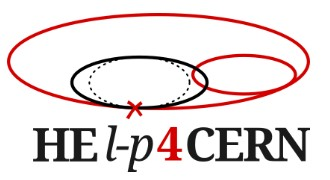
\includegraphics[width=1.5cm]{HELP4CERN.jpg}};
\end{tikzpicture}

\end{frame}
% --------------------------------------------------------------------------







% --------------------------------------------------------------------------
% Slide 15 
% --------------------------------------------------------------------------
\begin{frame}{Top-FCNC probes at \LHCmu{}: \(tq\gamma\) and \(tqZ\)}
	
\begin{columns}[T]
		
%================================================
% Left column: text
%================================================
\begin{column}{0.68\textwidth}
\small
\begin{itemize}\itemsep0.48em
\justifying
				
\item In the Standard Model, top-FCNC transitions are forbidden at tree level and remain highly suppressed at loop level by the GIM mechanism; any observable signal would therefore be a clean indication of physics beyond the Standard Model.
				
\item The key rare-top vertices are \(tq\gamma\) and \(tqZ\) with \(q=u,c\), naturally parameterized by anomalous couplings or SMEFT dimension-6 operators.
				
\item At \LHCmu{}, the large top sample, harder kinematics, and characteristic \(\mu p\) topology make anomalous single-top and associated production natural benchmarks for converting top statistics into BSM reach.
				
\end{itemize}
\end{column}
		
%================================================
% Right column: diagrams
%================================================
\begin{column}{0.47\textwidth}
\centering
			
%-----------------------------
% Diagram A: tqgamma / tqZ
%-----------------------------
%-----------------------------
% Diagram A: tqgamma and tqZ side by side
%-----------------------------
\begin{minipage}{\linewidth}
\centering
\begin{center}
\setlength{\fboxsep}{3pt}
\fcolorbox{black!40}{yellow!20}{%
\parbox{0.50\linewidth}{\centering\scriptsize\textbf{Top-FCNC at \LHCmu{}}}%
}
\end{center}
\vspace{-0.35em}
	
\begin{minipage}{0.48\linewidth}
\centering
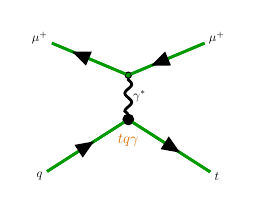
\begin{tikzpicture}[scale=0.45, transform shape]
\begin{feynman}
\vertex (muin)  at (-2.5,  1.95) {\(\mu^{+}\)};
\vertex (muout) at ( 2.5,  1.95) {\(\mu^{+}\)};
\vertex (qin)   at (-2.5, -1.95) {\(q\)};
\vertex (tout)  at ( 2.5, -1.95) {\(t\)};
				
\vertex [dot, fill=green!60!black, minimum size=5pt] (v1) at (0, 0.90) {};
\vertex [dot, fill=black, minimum size=8.5pt] (v2) at (0,-0.35) {};
				
\diagram*{
					(muin)  -- [anti fermion, draw=green!60!black, line width=1.0pt] (v1)
					-- [anti fermion, draw=green!60!black, line width=1.0pt] (muout),
					
					(v1)    -- [boson, edge label=\(\gamma^{\ast}\), line width=1.0pt] (v2),
					
					(qin)   -- [fermion, draw=green!60!black, line width=1.0pt] (v2)
					-- [fermion, draw=green!60!black, line width=1.0pt] (tout),
				};
\end{feynman}
\node[font=\large\bfseries,text=orange!85!black] at (0.0,-0.95) {\(tq\gamma\)};
\end{tikzpicture}
		
%\vspace{-0.2em}
%{\scriptsize \textcolor{orange!85!black}{\textbf{\(tq\gamma\)}}}

\end{minipage}
\hfill
\begin{minipage}{0.48\linewidth}
\centering
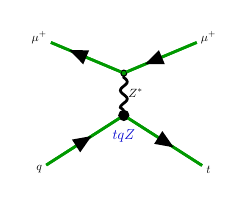
\begin{tikzpicture}[scale=0.43, transform shape]
\begin{feynman}
				\vertex (muin)  at (-2.5,  1.95) {\(\mu^{+}\)};
				\vertex (muout) at ( 2.5,  1.95) {\(\mu^{+}\)};
				\vertex (qin)   at (-2.5, -1.95) {\(q\)};
				\vertex (tout)  at ( 2.5, -1.95) {\(t\)};
				
				\vertex [dot, fill=green!60!black, minimum size=5pt] (v1) at (0, 0.90) {};
				\vertex [dot, fill=black, minimum size=8.5pt] (v2) at (0,-0.35) {};
				
				\diagram*{
					(muin)  -- [anti fermion, draw=green!60!black, line width=1.0pt] (v1)
					-- [anti fermion, draw=green!60!black, line width=1.0pt] (muout),
					
					(v1)    -- [boson, edge label=\(Z^{\ast}\), line width=1.0pt] (v2),
					
					(qin)   -- [fermion, draw=green!60!black, line width=1.0pt] (v2)
					-- [fermion, draw=green!60!black, line width=1.0pt] (tout),
				};
\end{feynman}
\node[font=\large\bfseries, text=blue!80!black] at (0.0,-0.95) {\(tqZ\)};

\end{tikzpicture}
		
%\vspace{-0.2em}
%{\scriptsize \textcolor{blue!80!black}{\textbf{\(tqZ\)}}}

\end{minipage}
	
\vspace{0.5em}
	
\justifying\scriptsize
Representative process: \(\mu^{+} q \to \mu^{+} t\), with \(q=u,c\).
Neutral-current exchange probes anomalous \(tq\gamma\) and \(tqZ\) couplings.
\end{minipage}
			
\end{column}
\end{columns}

\begin{center}
\setlength{\fboxsep}{6pt}
\fcolorbox{red!50!black}{red!10}{%
\parbox{0.88\linewidth}{%
\justifying\small
Improved sensitivity relative to the LHeC is expected at \LHCmu{}, but quantitative limits remain channel-dependent and require realistic event selections, detector modelling, and systematic-uncertainty estimates.
}%
}
\end{center}

%------------------------------------------------
% HELP4CERN logo overlay
%------------------------------------------------
\begin{tikzpicture}[remember picture,overlay]
\node[anchor=north east, xshift=-0.10cm, yshift=-1.25cm]
at (current page.north east)
{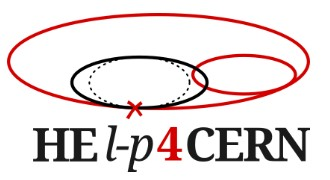
\includegraphics[width=1.5cm]{HELP4CERN.jpg}};
\end{tikzpicture}

\end{frame}
% --------------------------------------------------------------------------



\section{Beyond SM and long-term outlook}



% --------------------------------------------------------------------------
% Slide 16
% --------------------------------------------------------------------------
\begin{frame}{Why \LHCmu{} is also a distinctive BSM machine}
\begin{itemize}
\justifying 
\item $\mu^+p$ collisions provide a distinctive BSM environment: a point-like muon beam scatters from quarks and gluons at multi-TeV centre-of-mass energy. 
\item The key advantage is channel-specific: \(\mu q\) and \(\mu g\) initial states can directly probe new particles coupled to second-generation leptons, 
\[
\mu q \to X,
\qquad
\mu g \to X .
\]
\item This enables resonant single production of states that may be harder to isolate through pair production or inclusive searches at hadron colliders. 
\item The \LHCmu{} is naturally powerful for BSM scenarios tied to second-generation leptons. 
\item Representative examples include:
\begin{itemize}
\justifying
\item R-parity-violating squark searches,
\item color-octet muons (leptogluons),
\item excited leptons,
\item contact interactions,
\item and other muon-coupled new-physics scenarios.
\end{itemize}
\end{itemize}

\begin{tikzpicture}[remember picture,overlay]
\node[anchor=north east, xshift=-0.10cm, yshift=-1.25cm]
at (current page.north east)
{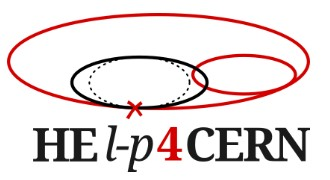
\includegraphics[width=1.5cm]{HELP4CERN.jpg}};
\end{tikzpicture}

%\vspace{0.3em}
%{\justifying \scriptsize
%\setlength{\fboxsep}{4pt}%
%\colorbox{green!15}{%
%\parbox{0.92\linewidth}{%
%Kingman Cheung and Zeren Simon Wang, \textit{Physics potential of a muon-proton collider}, Phys.\ Rev.\ D~103 (2021) 116009.%
%}%
%}%
%}

\end{frame}







% --------------------------------------------------------------------------
% Slide 17
% --------------------------------------------------------------------------
\begin{frame}{Representative BSM benchmarks: RPV squarks and color-octet muons}
	
\begin{columns}[T]%[T,onlytextwidth]
		
%================================================
% Left column: benchmark results
%================================================
\begin{column}{0.60\textwidth}
\footnotesize
\begin{itemize}\itemsep0.42em
\justifying
				
\item RPV SUSY: 
\(LQD\)-type operators can give resonant squark production in \(\mu q\) scattering. 
In favourable NC benchmark channels, 
\(\lambda'_{2j1}\sim 0.01\text{-}0.02\) can be tested for squark masses of 
\(1\)-\(3~\mathrm{TeV}\), approaching an order-of-magnitude improvement over LHC bounds in the on-shell regime.
				
\item Color-octet muon \(\mu_8\) / leptogluon: 
the direct \(\mu g\) initial state enables resonant single production,
\[
\mu g \to \mu_8 \to \mu g ,
\]
whereas \(pp\) searches mainly rely on pair production.

\end{itemize}



\vspace{0.10em}



%------------------------------------------------
% Yellow benchmark reach box
%------------------------------------------------
\begin{center}
\setlength{\fboxsep}{4pt}
\fcolorbox{black!35}{yellow!15}{%
\parbox{0.70\linewidth}{%
\centering\scriptsize
\textbf{Representative \(5\sigma\) reach for \(\mu_8\)}\\[0.45ex]
\begin{tabular}{lc}
HL-LHC & \(\sim 2.3~\mathrm{TeV}\) \\
\LHCmu{}, \(E_\mu=500~\mathrm{GeV}\) & \(\sim 3.0~\mathrm{TeV}\) \\
\LHCmu{}, \(E_\mu=1~\mathrm{TeV}\) & \(\sim 4.2~\mathrm{TeV}\)
\end{tabular}
}%
}
\end{center}

\vspace{0.10em}

%------------------------------------------------
% Red caution box
%------------------------------------------------
\begin{center}
\setlength{\fboxsep}{4pt}
\fcolorbox{red!50!black}{red!8}{%
\parbox{0.90\linewidth}{%
\justifying\scriptsize
These are representative benchmark studies. Final reach requires channel-specific selections, detector/MDI modelling, and systematic-uncertainty estimates.
}%
}
\end{center}

\end{column}



%================================================
% Right column: figures
%================================================
\begin{column}{0.50\textwidth}

\vspace{-0.5em}
\centering

%-----------------------------
% RPV figure
%-----------------------------
\begin{center}
\setlength{\fboxsep}{3pt}
\fcolorbox{black!40}{yellow!20}{%
\parbox{0.60\linewidth}{\centering\scriptsize\textbf{RPV squark coupling reach}}%
}
\end{center}
\vspace{-0.35em}


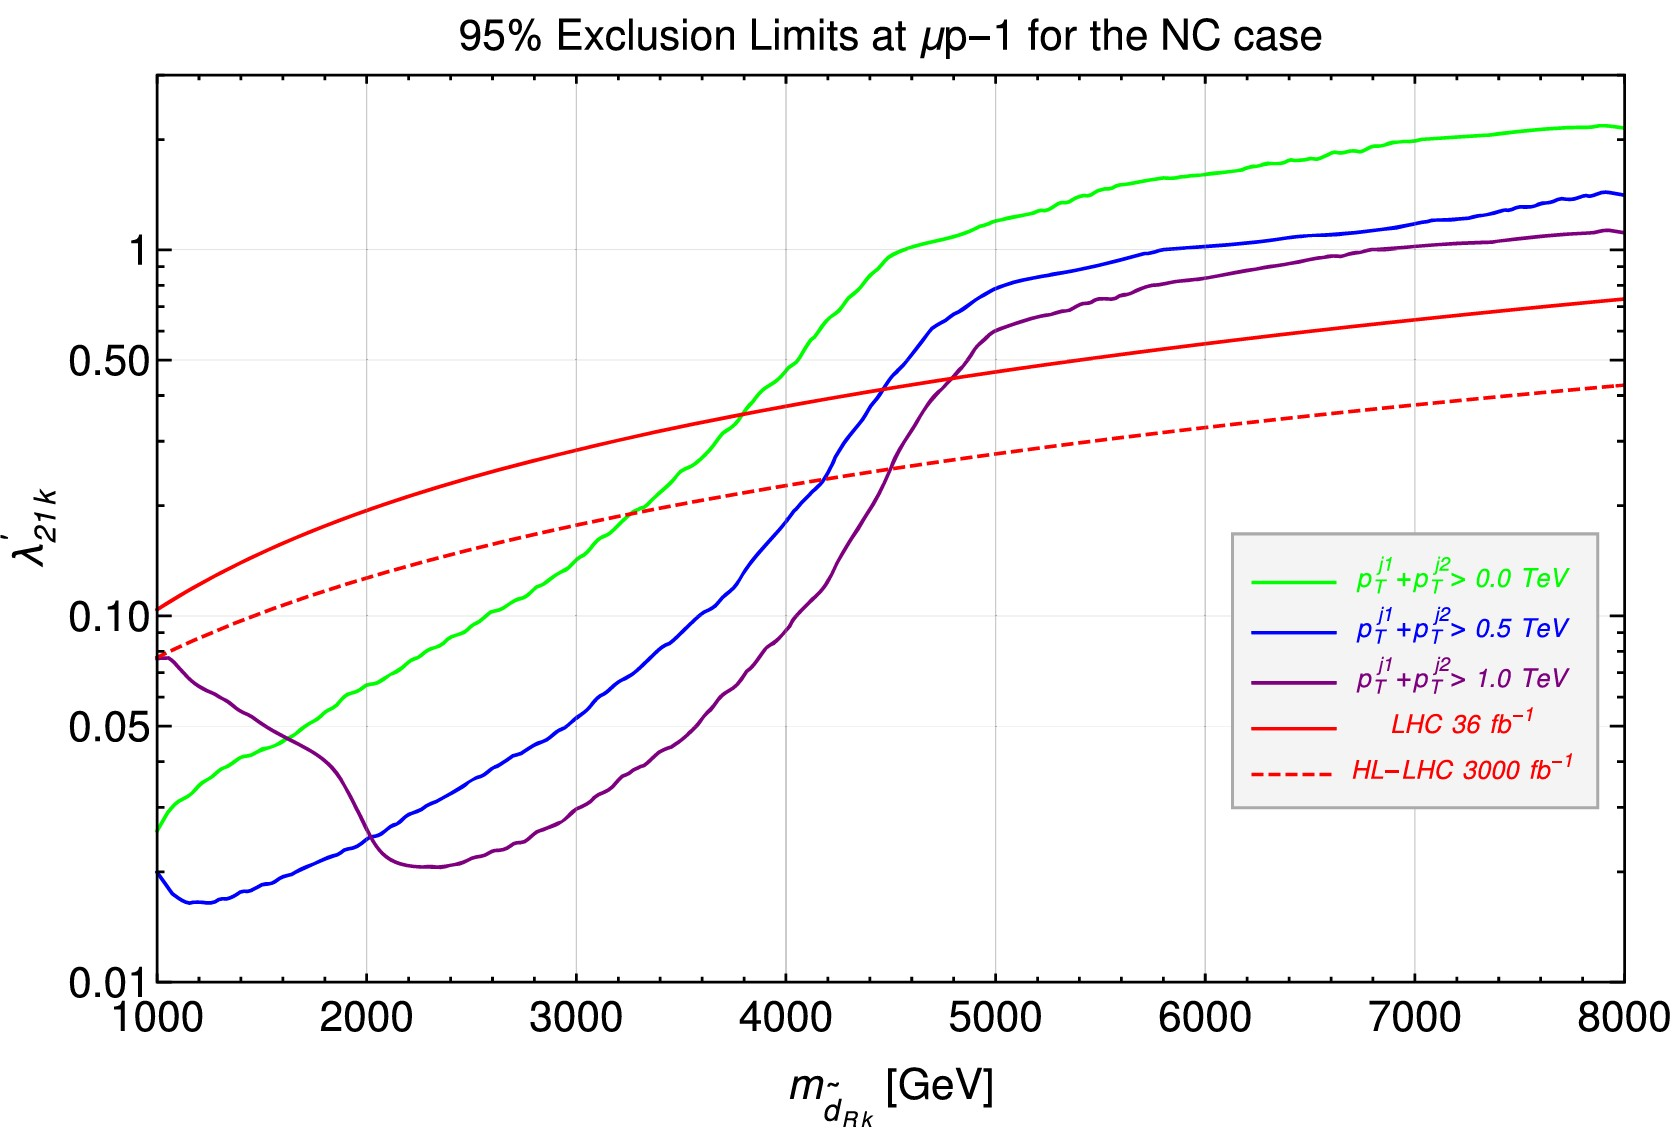
\includegraphics[
width=0.99\linewidth,
height=0.26\textheight,
keepaspectratio
]{exclusion_limits.jpg}



\vspace{0.18em}

%-----------------------------
% mu8 figure
%-----------------------------
\begin{center}
\setlength{\fboxsep}{3pt}
\fcolorbox{black!40}{yellow!20}{%
\parbox{0.60\linewidth}{\centering\scriptsize\textbf{Color-octet muon \(\mu_8\) reach}}%
}
\end{center}

\vspace{-0.35em}

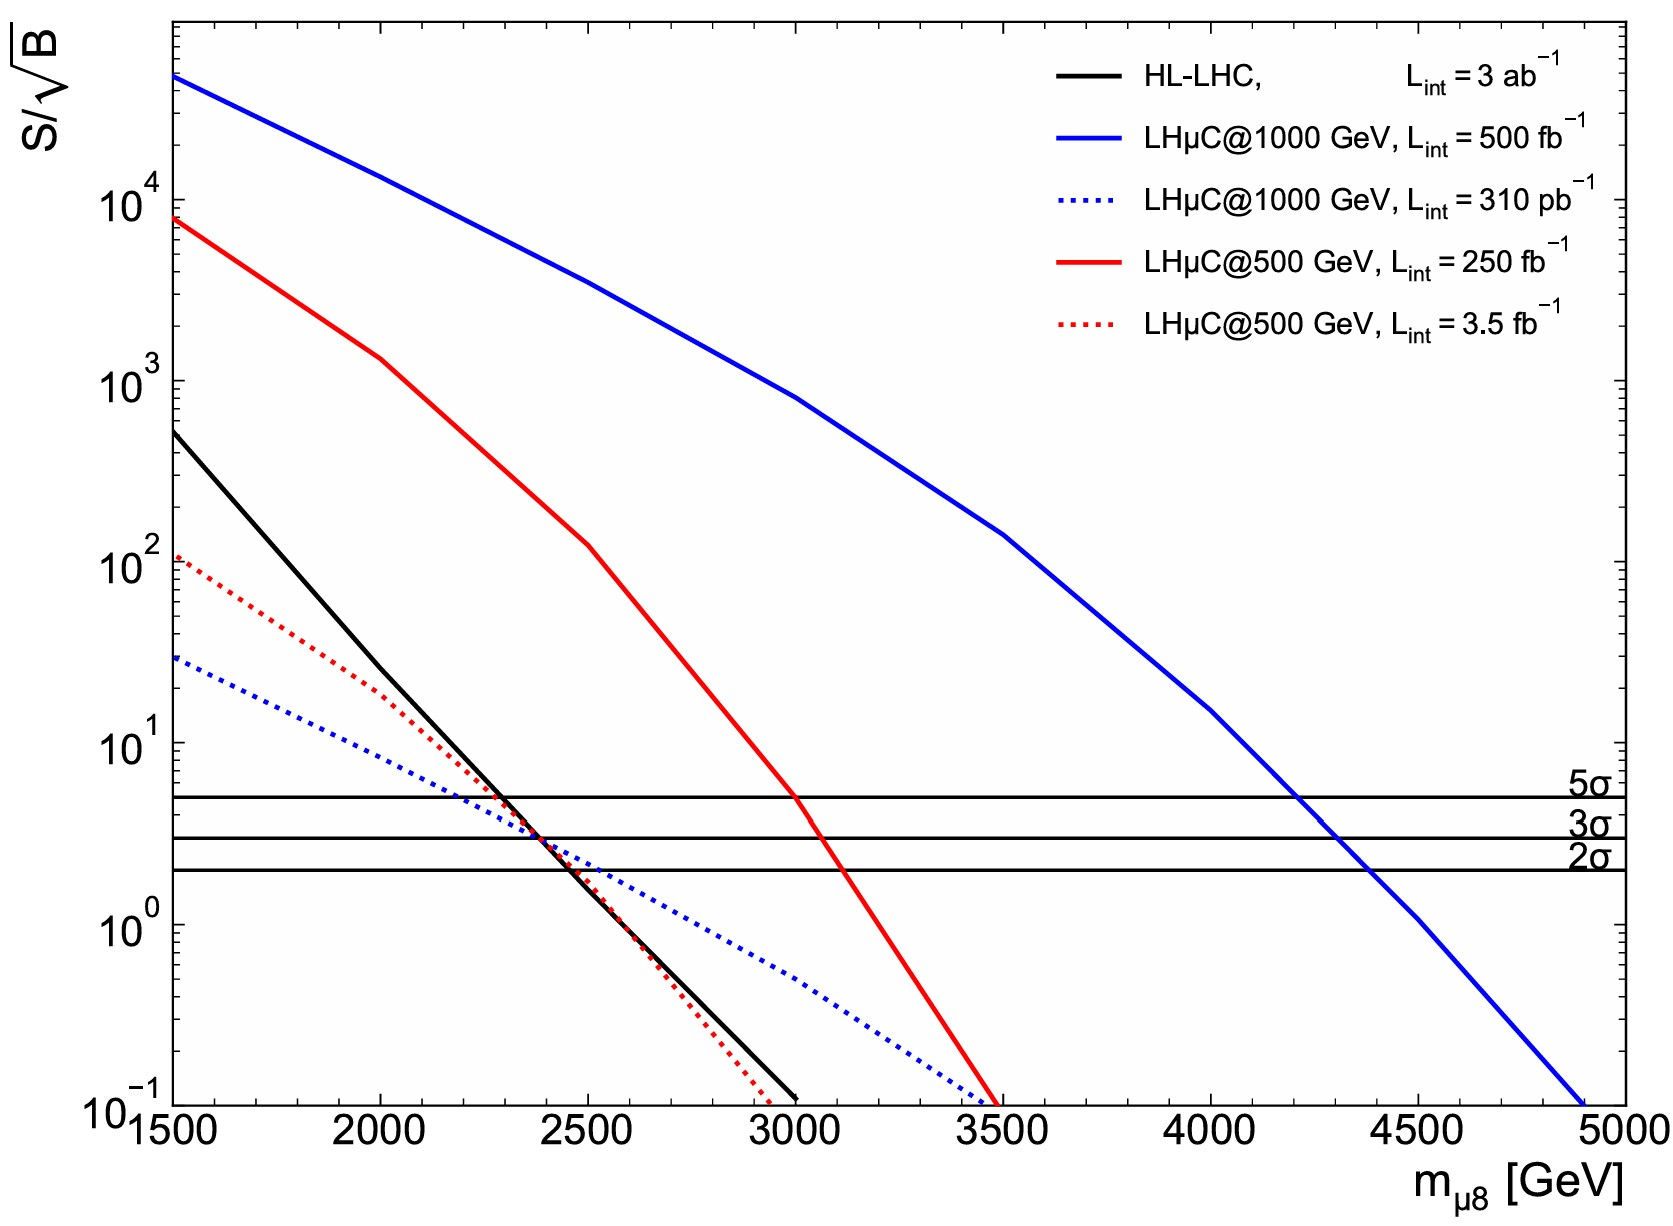
\includegraphics[
width=0.99\linewidth,
height=0.26\textheight,
keepaspectratio
]{mu8.jpg}

\vspace{0.05em}

\justifying\scriptsize
The key advantage is the resonant \(\mu g\) channel, which is absent in \(pp\) pair-production searches.

\end{column}

\end{columns}


%------------------------------------------------
% HELP4CERN logo overlay
%------------------------------------------------
\begin{tikzpicture}[remember picture,overlay]
\node[anchor=north east, xshift=-0.10cm, yshift=-1.25cm]
at (current page.north east)
{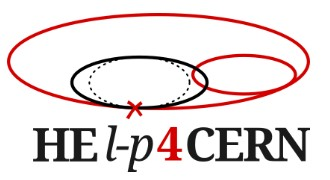
\includegraphics[width=1.5cm]{HELP4CERN.jpg}};
\end{tikzpicture}

\vspace{0.15em}
	
%------------------------------------------------
% Reference box
%------------------------------------------------
%\begin{center}
%\setlength{\fboxsep}{4pt}
%\colorbox{green!15}{%
%\parbox{0.90\linewidth}{%
%\scriptsize
%K. Cheung and Z. S. Wang, \textit{Physics potential of a muon-proton collider},
%Phys.\ Rev.\ D~103 (2021) 116009; HELP4CERN white-paper draft benchmark studies.
%}%
%}
%\end{center}
	
\end{frame}
% --------------------------------------------------------------------------






% --------------------------------------------------------------------------
% Slide 18
% --------------------------------------------------------------------------
\begin{frame}{Toward FCC-\(\mu h\): final outlook and take-home points}
\begin{columns}[T]
\begin{column}{0.99\textwidth}
\begin{itemize}
\justifying
\item The long-term perspective goes well beyond the 3.7 TeV baseline.
\item The FCC-hh era is explicitly connected to a future high-energy $\mu p$ option, turning the current \LHCmu{} concept into a stepping stone toward even more powerful HET and BSM programmes.
\item In particular, a future FCC-$\mu h$ machine would extend:
\begin{itemize}
\justifying
\item Higgs statistics and coupling reach,
\item top and rare-top production,
\item high-mass electroweak and $\gamma\gamma$ studies,
\item and resonant BSM sensitivity.
\end{itemize}
\end{itemize}

\begin{block}{HET@\LHCmu{}}
\small
\justifying
(1) \LHCmu{} is a serious HET factory; \\
(2) the top sector is one of its clearest near-term strengths; \\
(3) Higgs, EW, EFT, and $\gamma\gamma$ studies are all strongly motivated; \\
(4) the concept also provides a natural bridge toward FCC-era $\mu p$ physics.
\end{block}

\end{column}
\end{columns}
\begin{tikzpicture}[remember picture,overlay]
\node[anchor=north east, xshift=-0.10cm, yshift=-1.25cm]
at (current page.north east)
{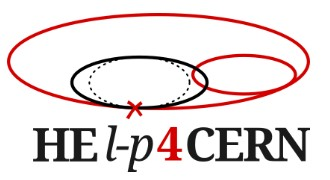
\includegraphics[width=1.5cm]{HELP4CERN.jpg}};
\end{tikzpicture}
\end{frame}





% --------------------------------------------------------------------------
% Summary and conclusions
% --------------------------------------------------------------------------
\begin{frame}{Summary and conclusions}

\vspace{0.35em}

%------------------------------------------------
% Four-pillar physics summary
%------------------------------------------------
\begin{columns}[T,onlytextwidth]

%================================================
% Left pair
%================================================
\begin{column}{0.49\textwidth}

% QCD / DIS box
\setlength{\fboxsep}{5pt}
\fcolorbox{green!50!black}{green!8}{%
\parbox{0.96\linewidth}{%
\scriptsize
\textbf{\textcolor{green!45!black}{QCD \& DIS frontier}}\\[0.4ex]
\justifying
Multi-TeV \(\mu p\) scattering extends the accessible \((x,Q^2)\) plane well beyond HERA and the EIC/LHeC, strengthening the PDF, small-\(x\), and \(\alpha_s\) programme.
}%
}

\vspace{0.55em}

% Higgs / EW box
\fcolorbox{blue!55!black}{blue!5}{%
\parbox{0.96\linewidth}{%
\scriptsize
\textbf{\textcolor{blue!70!black}{Higgs--EW precision}}\\[0.4ex]
\justifying
Large CC/NC Higgs samples enable concrete coupling studies; the \(h\to b\bar b\) benchmark reaches sub-percent sensitivity to \(g_{hbb}\), while EW/SMEFT observables gain a larger high-\(Q^2\) lever arm.
}%
}

\end{column}

%================================================
% Right pair
%================================================
\begin{column}{0.49\textwidth}

% Top box
\setlength{\fboxsep}{5pt}
\fcolorbox{red!55!black}{red!6}{%
\parbox{0.96\linewidth}{%
\scriptsize
\textbf{\textcolor{red!70!black}{Top and rare-top physics}}\\[0.4ex]
\justifying
The top sector gives the clearest rate gain: already the 500~GeV \LHCmu{} benchmark enhances \(t\bar t\) production by \(\sim32\) relative to the 50~GeV LHeC case, motivating precision top and FCNC studies.
}%
}

\vspace{0.55em}

% gamma gamma / BSM box
\fcolorbox{orange!70!black}{orange!8}{%
\parbox{0.96\linewidth}{%
\scriptsize
\textbf{\textcolor{orange!80!black}{\(\gamma\gamma\) and BSM portals}}\\[0.4ex]
\justifying
Photon-induced channels provide high-statistics \(\tau^+\tau^-\) samples and high-mass \(WW,ZZ,t\bar t\) probes, while direct \(\mu q\) and \(\mu g\) portals target RPV squarks, color-octet muons, and other muon-coupled BSM states.
}%
}

\end{column}

\end{columns}

\vspace{0.55em}

%------------------------------------------------
% Final take-home message
%------------------------------------------------
\begin{center}
\setlength{\fboxsep}{6pt}
\fcolorbox{black!45}{yellow!25}{%
\parbox{0.92\linewidth}{%
\justifying \small
Looking ahead:  
\LHCmu{} is not simply an energy upgrade of the LHeC; it opens a 
multi-TeV lepton-hadron regime where QCD, Higgs, electroweak, top, photon-induced, and several BSM studies become quantitatively competitive.
}%
}
\end{center}
	
%\vspace{0.15em}
	
%\begin{center}
%\scriptsize
%\textcolor{black!65}{Results shown here are benchmark physics projections; detector, MDI, and systematic studies remain essential for final sensitivity estimates.}
%\end{center}


%------------------------------------------------
% HELP4CERN logo overlay
%------------------------------------------------
\begin{tikzpicture}[remember picture,overlay]
\node[anchor=north east, xshift=-0.10cm, yshift=-1.25cm]
at (current page.north east)
{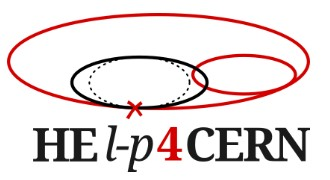
\includegraphics[width=1.5cm]{HELP4CERN.jpg}};
\end{tikzpicture}
	
\end{frame}
% --------------------------------------------------------------------------









% --------------------------------------------------------------------------
% Slide 20
% --------------------------------------------------------------------------
\begin{frame}[plain]
\begin{center}

\includegraphics[width=0.85\paperwidth,height=0.85\paperheight,keepaspectratio]{Thank_You_2.jpg}
\end{center}
\end{frame}












% --------------------------------------------------------------------------
% Backup slide
% --------------------------------------------------------------------------
\begin{frame}{The HELP4CERN collaboration}
	
\begin{columns}[T] % [T,onlytextwidth]
	
%========================================
% Left column
%========================================
\begin{column}{0.55\textwidth}

\setbeamercolor{greenbox}{bg=green!10,fg=black}
\begin{beamercolorbox}[wd=\linewidth,sep=0.9em,rounded=true,shadow=true]{greenbox}
\justifying
\small
\textbf{HELP4CERN} collaboration focuses on the physics case for
high-energy, high-luminosity lepton-hadron colliders at CERN.

\begin{itemize}
\justifying
\small
\item assess the physics potential of future lepton-hadron collider options,
\item develop benchmark studies for Higgs, electroweak, top, QCD, and BSM physics,
\item provide a common framework for phenomenology, detector studies, and future projections,
\item new contributions and physics studies are very welcome,
\end{itemize}

\textbf{Contact:} \texttt{help-4-cern@cern.ch}\\
\textbf{Visit:} \texttt{https://help4cern.web.cern.ch}
\end{beamercolorbox}
\end{column}
		
%========================================
% Right column
%========================================
\begin{column}{0.50\textwidth}
\centering
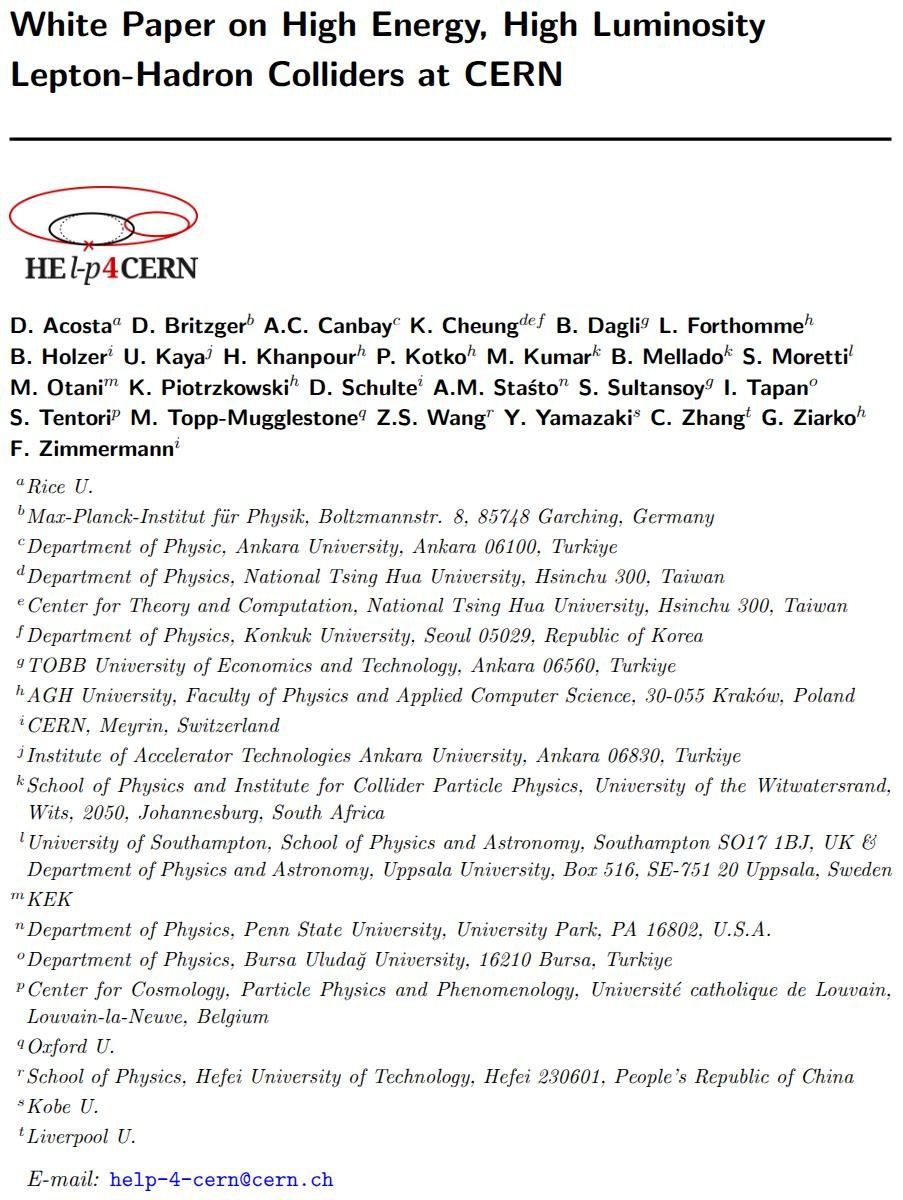
\includegraphics[width=\linewidth]{White_Paper.jpg}
\end{column}

\end{columns}
	
\end{frame}








% --------------------------------------------------------------------------
% Slide 13
% --------------------------------------------------------------------------

% --------------------------------------------------------------------------
% Merged gamma-gamma summary slide
% --------------------------------------------------------------------------
\begin{frame}{Exclusive $\gamma\gamma$ channels: electroweak, top, and BSM reach}
	
	\centering
	%	\vspace{-0.35em}
	
	\begin{tikzpicture}[x=1cm,y=1cm]
		
		%------------------------------------------------
		% Styles
		%------------------------------------------------
		\tikzset{
			connector/.style={
				draw=blue!65!black,
				line width=1.0pt
			},
			hubbox/.style={
				rounded corners=6pt,
				draw=blue!65!black,
				line width=1.1pt,
				fill=white,
				minimum width=2.9cm,
				minimum height=2.0cm,
				inner sep=3pt,
				align=center
			},
			boxww/.style={
				rounded corners=9pt,
				draw=green!50!black,
				line width=1.15pt,
				fill=green!10,
				minimum width=3.85cm,
				minimum height=2.75cm,
				text width=3.20cm,
				align=center,
				inner sep=4pt
			},
			boxzz/.style={
				rounded corners=9pt,
				draw=violet!55!black,
				line width=1.15pt,
				fill=violet!10,
				minimum width=3.85cm,
				minimum height=2.75cm,
				text width=3.20cm,
				align=center,
				inner sep=4pt
			},
			boxtt/.style={
				rounded corners=9pt,
				draw=orange!70!black,
				line width=1.15pt,
				fill=orange!12,
				minimum width=3.85cm,
				minimum height=2.75cm,
				text width=3.20cm,
				align=center,
				inner sep=4pt
			},
			boxbsm/.style={
				rounded corners=9pt,
				draw=red!65!black,
				line width=1.15pt,
				fill=red!10,
				minimum width=3.85cm,
				minimum height=2.75cm,
				text width=3.20cm,
				align=center,
				inner sep=4pt
			},
			takehome/.style={
				rounded corners=5pt,
				draw=red!60!black,
				line width=0.95pt,
				fill=red!8,
				text width=11.1cm,
				minimum height=0.82cm,
				align=center,
				inner sep=3.5pt
			}
		}
		
		%------------------------------------------------
		% Central hub
		%------------------------------------------------
		\node[hubbox] (hub) at (0,0.00) {%
			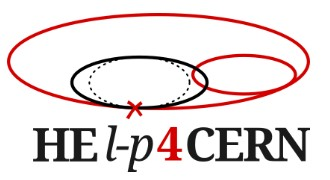
\includegraphics[width=2.05cm]{HELP4CERN.jpg}\\[-0.15em]
			{\scriptsize \textbf{Exclusive high-energy}}\\[-0.05em]
			{\scriptsize \textbf{$\gamma\gamma$ programme}}
		};
		
		%------------------------------------------------
		% Outer nodes
		%------------------------------------------------
		\node[boxww] (ww) at (-4.15,1.65) {%
			{\bfseries \small $\gamma\gamma\to W^+W^-$}\\[0.20em]
			%			{\footnotesize largest EW benchmark;}\\
			{\footnotesize Strong aQGC sensitivity comes from}\\
			{\footnotesize the high-$M_{WW}$ tail}\\[0.15em]
			%			{\footnotesize $\sigma_{\rm el}\simeq 0.166$ pb at 3.7 TeV}
		};
		
		\node[boxzz] (zz) at (4.15,1.65) {%
			{\bfseries \small $\gamma\gamma\to ZZ$}\\[0.20em]
			{\footnotesize Loop-induced in the SM;}\\
			{\footnotesize clean probe of high-mass}\\
			{\footnotesize electroweak dynamics}\\[0.15em]
			%			{\footnotesize $\sigma_{\rm el}\simeq 0.284$ fb at 3.7 TeV}
		};
		
		\node[boxtt] (tt) at (-4.15,-1.85) {%
			{\bfseries \small $\gamma\gamma\to t\bar t$}\\[0.20em]
			{\footnotesize Probes heavy thresholds}\\
			{\footnotesize and top-sector dynamics}\\
			{\footnotesize in exclusive topology}\\[0.15em]
			%			{\footnotesize $\sigma_{\rm el}\simeq 0.486$ fb at 3.7 TeV}
		};
		
		\node[boxbsm] (bsm) at (4.15,-1.85) {%
			{\bfseries \small Exclusive BSM pairs}\\[0.20em]
			%			{\footnotesize same framework extends to}\\
			{\footnotesize Charged states such as}\\
			{\footnotesize higgsinos and sleptons}\\[0.15em]
			%			{\footnotesize qualitative opportunity; no rate quoted here}
		};
		
		%------------------------------------------------
		% Connectors
		%------------------------------------------------
		\draw[connector] (hub.north west) .. controls (-1.1,0.95) and (-2.4,1.35) .. (ww.east);
		\draw[connector] (hub.north east) .. controls ( 1.1,0.95) and ( 2.4,1.35) .. (zz.west);
		\draw[connector] (hub.south west) .. controls (-1.1,-0.85) and (-2.4,-1.35) .. (tt.east);
		\draw[connector] (hub.south east) .. controls ( 1.1,-0.85) and ( 2.4,-1.35) .. (bsm.west);
		
		%------------------------------------------------
		% Inset Feynman diagram: gamma gamma -> W+ W-
		%------------------------------------------------
		\begin{scope}[
			shift={(0,2.18)},
			scale=0.255,
			transform shape,
			line cap=round,
			line join=round,
			>=Triangle
			]
			
			% Coordinates
			\coordinate (wwEin)   at (-4.00,  2.25);
			\coordinate (wwEv)    at (-1.25,  1.25);
			\coordinate (wwEout)  at ( 2.10,  2.15);
			
			\coordinate (wwPin)   at (-4.00, -2.75);
			\coordinate (wwPv)    at (-1.05, -1.85);
			\coordinate (wwPout)  at ( 2.20, -2.75);
			
			\coordinate (wwB)     at ( 0.55, -0.05);
			\def\wwBr{0.35}
			
			\coordinate (wwGtopEnd) at ( 0.27,  0.17);
			\coordinate (wwGbotEnd) at ( 0.24, -0.36);
			
			\coordinate (wwWupA)  at ( 0.86,  0.10);
			\coordinate (wwWupB)  at ( 2.55,  0.78);
			
			\coordinate (wwWdnA)  at ( 0.86, -0.20);
			\coordinate (wwWdnB)  at ( 2.55, -0.72);
			
			% Electron line
			\draw[line width=0.9pt] (wwEin) -- (wwEv) -- (wwEout);
			
			\draw[-{Triangle[length=5.8pt,width=7.0pt]}, line width=0.5pt]
			(-2.95,1.87) -- (-2.10,1.56);
			
			\draw[-{Triangle[length=5.8pt,width=7.0pt]}, line width=0.5pt]
			(0.10,1.60) -- (0.95,1.83);
			
			% Proton line
			\draw[line width=1.4pt] (wwPin) -- (wwPv) -- (wwPout);
			
			\draw[-{Triangle[length=6.0pt,width=5.2pt]}, line width=1.0pt]
			(-3.05,-2.46) -- (-2.10,-2.17);
			
			\draw[-{Triangle[length=6.0pt,width=5.2pt]}, line width=1.0pt]
			(0.05,-2.16) -- (1.00,-2.42);
			
			% Off-shell photons
			\draw[
			decorate,
			decoration={snake, amplitude=2.8pt, segment length=8pt},
			line width=1.2pt
			] (wwEv) -- (wwGtopEnd);
			
			\draw[
			decorate,
			decoration={snake, amplitude=2.8pt, segment length=8pt},
			line width=1.2pt
			] (wwPv) -- (wwGbotEnd);
			
			% Central red striped effective-interaction blob
			\begin{scope}
				\clip (wwB) circle (\wwBr);
				\fill[white] (wwB) circle (\wwBr);
				
				\foreach \t in {-1.30,-1.15,...,1.30}{
					\draw[red!85!black, line width=1.3pt]
					($(wwB)+(\t,-1.20)$) -- ($(wwB)+(\t+1.60,0.40)$);
				}
			\end{scope}
			
			\draw[red!85!black, line width=1.5pt] (wwB) circle (\wwBr);
			
			% W bosons
			\draw[line width=1.2pt, dashed] (wwWupA) -- (wwWupB);
			\draw[line width=1.2pt, dashed] (wwWdnA) -- (wwWdnB);
			
			\draw[-{Triangle[length=5.4pt,width=4.5pt]}, line width=0.50pt]
			(2.02,0.56) -- (1.52,0.36);
			
			\draw[-{Triangle[length=5.4pt,width=4.5pt]}, line width=0.50pt]
			(2.02,-0.56) -- (1.52,-0.40);
			
			% Labels
			\node[font=\fontsize{20}{22}\selectfont] at (-4.40,  2.75) {$\ell$};
			\node[font=\fontsize{20}{22}\selectfont] at ( 2.42,  2.65) {$\ell$};
			
			\node[font=\fontsize{20}{22}\selectfont] at (-4.42, -3.05) {$p$};
			\node[font=\fontsize{20}{22}\selectfont] at ( 2.95, -3.12) {$p^{(*)}$};
			
			\node[font=\fontsize{24}{26}\selectfont] at (-1.55,  0.33) {$\gamma^{*}$};
			\node[font=\fontsize{24}{26}\selectfont] at (-1.60, -0.92) {$\gamma^{*}$};
			
			\node[font=\fontsize{24}{26}\selectfont, anchor=west] at ( 2.92,  0.96) {$W^{+}$};
			\node[font=\fontsize{24}{26}\selectfont, anchor=west] at ( 2.92, -0.96) {$W^{-}$};
			
		\end{scope}
		
		%------------------------------------------------
		% Inset Feynman diagram: gamma gamma -> Htilde+ Htilde-
		%------------------------------------------------
		\begin{scope}[
			shift={(0,-2.45)},
			scale=0.220,
			transform shape,
			line cap=round,
			line join=round,
			>=Triangle
			]
			
			% Coordinates
			\coordinate (hhLin)   at (-4.00,  2.70);
			\coordinate (hhLv)    at (-0.90,  1.95);
			\coordinate (hhLout)  at ( 3.50,  2.70);
			
			\coordinate (hhPin)   at (-4.00, -3.20);
			\coordinate (hhPv)    at (-0.90, -2.45);
			\coordinate (hhPout)  at ( 3.50, -3.20);
			
			\coordinate (hhTopJ)  at ( 1.25,  0.35);
			\coordinate (hhBotJ)  at ( 1.25, -1.05);
			
			\coordinate (hhTopR)  at ( 4.05,  0.35);
			\coordinate (hhBotR)  at ( 4.05, -1.05);
			
			% Upper lepton line
			\draw[line width=0.9pt] (hhLin) -- (hhLv) -- (hhLout);
			
			\draw[-{Triangle[length=5.8pt,width=7.0pt]}, line width=0.5pt]
			(-2.95,2.45) -- (-2.05,2.23);
			
			\draw[-{Triangle[length=5.8pt,width=7.0pt]}, line width=0.5pt]
			(0.80,2.25) -- (1.70,2.47);
			
			% Lower proton line
			\draw[line width=1.4pt] (hhPin) -- (hhPv) -- (hhPout);
			
			\draw[-{Triangle[length=6.0pt,width=5.2pt]}, line width=1.0pt]
			(-2.95,-2.93) -- (-2.00,-2.70);
			
			\draw[-{Triangle[length=6.0pt,width=5.2pt]}, line width=1.0pt]
			(0.80,-2.70) -- (1.75,-2.93);
			
			% Off-shell photons
			\draw[
			decorate,
			decoration={snake, amplitude=2.8pt, segment length=8pt},
			line width=1.2pt
			] (hhLv) -- (hhTopJ);
			
			\draw[
			decorate,
			decoration={snake, amplitude=2.8pt, segment length=8pt},
			line width=1.2pt
			] (hhPv) -- (hhBotJ);
			
			% Double-dashed interaction structure
			\draw[line width=1.2pt, dash pattern=on 6pt off 5pt] (1.25, 0.44) -- (4.05, 0.44);
			\draw[line width=1.2pt, dash pattern=on 6pt off 5pt] (1.25, 0.26) -- (4.05, 0.26);
			
			\draw[line width=1.2pt, dash pattern=on 6pt off 5pt] (1.25,-0.96) -- (4.05,-0.96);
			\draw[line width=1.2pt, dash pattern=on 6pt off 5pt] (1.25,-1.14) -- (4.05,-1.14);
			
			\draw[line width=1.2pt, dash pattern=on 6pt off 5pt] (1.16, 0.35) -- (1.16,-1.05);
			\draw[line width=1.2pt, dash pattern=on 6pt off 5pt] (1.34, 0.35) -- (1.34,-1.05);
			
			% Labels
			\node[font=\fontsize{20}{22}\selectfont] at (-4.40,  3.10) {$\ell$};
			\node[font=\fontsize{20}{22}\selectfont] at ( 3.95,  3.10) {$\ell$};
			
			\node[font=\fontsize{20}{22}\selectfont] at (-4.42, -3.72) {$p$};
			\node[font=\fontsize{20}{22}\selectfont] at ( 4.25, -3.95) {$p^{(*)}$};
			
			\node[font=\fontsize{26}{28}\selectfont] at (-0.35,  0.55) {$\gamma^{*}$};
			\node[font=\fontsize{26}{28}\selectfont] at (-0.35, -1.10) {$\gamma^{*}$};
			
			\node[font=\fontsize{24}{26}\selectfont, anchor=west] at (4.45,  0.45) {$\widetilde{H}^{+}$};
			\node[font=\fontsize{24}{26}\selectfont, anchor=west] at (4.45, -1.15) {$\widetilde{H}^{-}$};
			
		\end{scope}
		
		%------------------------------------------------
		% Take-home message
		%------------------------------------------------
		\node[takehome] at (0,-4.00) {%
			{\justifying\scriptsize Beyond $\tau^+\tau^-$, the high-energy $\gamma\gamma$ programme at LH$\mu$C spans
				electroweak, top, and BSM-sensitive channels in a clean exclusive environment.}
		};
		
	\end{tikzpicture}
	
\end{frame}
% --------------------------------------------------------------------------





\end{document}







\begin{frame}
	\centering
	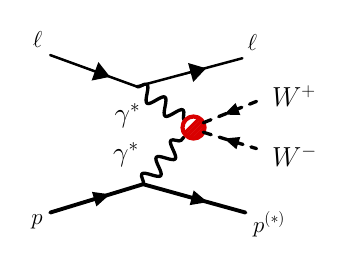
\begin{tikzpicture}[
		x=1cm,
		y=1cm,
		scale=0.40,
		transform shape,
		line cap=round,
		line join=round,
		>=Triangle
		]
		
		%------------------------------------------------------------------
		% Coordinates
		%------------------------------------------------------------------
		\coordinate (eIn)   at (-4.00,  2.25);
		\coordinate (eV)    at (-1.25,  1.25);
		\coordinate (eOut)  at ( 2.10,  2.15);
		
		\coordinate (pIn)   at (-4.00, -2.75);
		\coordinate (pV)    at (-1.05, -1.85);
		\coordinate (pOut)  at ( 2.20, -2.75);
		
		\coordinate (B)     at ( 0.55, -0.05);
		\def\Br{0.35}
		
		\coordinate (gTopEnd) at ( 0.27,  0.17);
		\coordinate (gBotEnd) at ( 0.24, -0.36);
		
		% Shortened W lines so they do not run into the labels
		\coordinate (WUpA)  at ( 0.86,  0.10);
		\coordinate (WUpB)  at ( 2.55,  0.78);
		
		\coordinate (WDnA)  at ( 0.86, -0.20);
		\coordinate (WDnB)  at ( 2.55, -0.72);
		
		%------------------------------------------------------------------
		% Electron line
		%------------------------------------------------------------------
		\draw[line width=0.9pt] (eIn) -- (eV) -- (eOut);
		
		% Electron arrows
		\draw[-{Triangle[length=5.8pt,width=7.0pt]}, line width=0.5pt]
		(-2.95,1.87) -- (-2.10,1.56);
		
		\draw[-{Triangle[length=5.8pt,width=7.0pt]}, line width=0.5pt]
		(0.10,1.60) -- (0.95,1.83);
		
		%------------------------------------------------------------------
		% Proton line
		%------------------------------------------------------------------
		\draw[line width=1.4pt] (pIn) -- (pV) -- (pOut);
		
		% Proton arrows
		\draw[-{Triangle[length=6.0pt,width=5.2pt]}, line width=1.0pt]
		(-3.05,-2.46) -- (-2.10,-2.17);
		
		\draw[-{Triangle[length=6.0pt,width=5.2pt]}, line width=1.0pt]
		(0.05,-2.16) -- (1.00,-2.42);
		
		%------------------------------------------------------------------
		% Off-shell photons
		%------------------------------------------------------------------
		\draw[
		decorate,
		decoration={snake, amplitude=2.8pt, segment length=8pt},
		line width=1.2pt
		] (eV) -- (gTopEnd);
		
		\draw[
		decorate,
		decoration={snake, amplitude=2.8pt, segment length=8pt},
		line width=1.2pt
		] (pV) -- (gBotEnd);
		
		%------------------------------------------------------------------
		% Central red striped effective-interaction blob
		%------------------------------------------------------------------
		\begin{scope}
			\clip (B) circle (\Br);
			\fill[white] (B) circle (\Br);
			
			% red diagonal hatching
			\foreach \t in {-1.30,-1.15,...,1.30}{
				\draw[red!85!black, line width=1.3pt]
				($(B)+(\t,-1.20)$) -- ($(B)+(\t+1.60,0.40)$);
			}
		\end{scope}
		
		\draw[red!85!black, line width=1.5pt] (B) circle (\Br);
		
		%------------------------------------------------------------------
		% W bosons: dashed lines, arrows pointing toward the blob
		%------------------------------------------------------------------
		\draw[line width=1.2pt, dashed] (WUpA) -- (WUpB);
		\draw[line width=1.2pt, dashed] (WDnA) -- (WDnB);
		
		% W arrows pointing leftward toward the central blob
		\draw[-{Triangle[length=5.4pt,width=4.5pt]}, line width=0.50pt]
		(2.02,0.56) -- (1.52,0.36);
		
		\draw[-{Triangle[length=5.4pt,width=4.5pt]}, line width=0.50pt]
		(2.02,-0.56) -- (1.52,-0.40);
		
		%------------------------------------------------------------------
		% Labels
		%------------------------------------------------------------------
		\node[font=\fontsize{20}{22}\selectfont] at (-4.40,  2.75) {$\ell$};
		\node[font=\fontsize{20}{22}\selectfont] at ( 2.42,  2.65) {$\ell$};
		
		\node[font=\fontsize{20}{22}\selectfont] at (-4.42, -3.05) {$p$};
		\node[font=\fontsize{20}{22}\selectfont] at ( 2.95, -3.12) {$p^{(*)}$};
		
		\node[font=\fontsize{24}{26}\selectfont] at (-1.55,  0.33) {$\gamma^{*}$};
		\node[font=\fontsize{24}{26}\selectfont] at (-1.60, -0.92) {$\gamma^{*}$};
		
		% Moved farther right so dashed lines do not cross the labels
		\node[font=\fontsize{24}{26}\selectfont, anchor=west] at ( 2.92,  0.96) {$W^{+}$};
		\node[font=\fontsize{24}{26}\selectfont, anchor=west] at ( 2.92, -0.96) {$W^{-}$};
		
	\end{tikzpicture}
\end{frame}




\begin{frame}
	\centering
	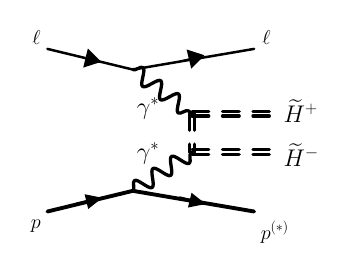
\begin{tikzpicture}[
		x=1cm,
		y=1cm,
		scale=0.35,
		transform shape,
		line cap=round,
		line join=round,
		>=Triangle
		]
		
		%------------------------------------------------------------------
		% Coordinates
		%------------------------------------------------------------------
		\coordinate (lIn)   at (-4.00,  2.70);
		\coordinate (lV)    at (-0.90,  1.95);
		\coordinate (lOut)  at ( 3.50,  2.70);
		
		\coordinate (pIn)   at (-4.00, -3.20);
		\coordinate (pV)    at (-0.90, -2.45);
		\coordinate (pOut)  at ( 3.50, -3.20);
		
		% Photon end points / left junctions of the double-dashed structure
		\coordinate (TopJ)  at ( 1.25,  0.35);
		\coordinate (BotJ)  at ( 1.25, -1.05);
		
		% Right ends of the double-dashed structure
		\coordinate (TopR)  at ( 4.05,  0.35);
		\coordinate (BotR)  at ( 4.05, -1.05);
		
		%------------------------------------------------------------------
		% Upper lepton line
		%------------------------------------------------------------------
		\draw[line width=0.9pt] (lIn) -- (lV) -- (lOut);
		
		% Lepton arrows
		\draw[-{Triangle[length=5.8pt,width=7.0pt]}, line width=0.5pt]
		(-2.95,2.45) -- (-2.05,2.23);
		
		\draw[-{Triangle[length=5.8pt,width=7.0pt]}, line width=0.5pt]
		(0.80,2.25) -- (1.70,2.47);
		
		%------------------------------------------------------------------
		% Lower proton line
		%------------------------------------------------------------------
		\draw[line width=1.4pt] (pIn) -- (pV) -- (pOut);
		
		% Proton arrows
		\draw[-{Triangle[length=6.0pt,width=5.2pt]}, line width=1.0pt]
		(-2.95,-2.93) -- (-2.00,-2.70);
		
		\draw[-{Triangle[length=6.0pt,width=5.2pt]}, line width=1.0pt]
		(0.80,-2.70) -- (1.75,-2.93);
		
		%------------------------------------------------------------------
		% Off-shell photons
		%------------------------------------------------------------------
		\draw[
		decorate,
		decoration={snake, amplitude=2.8pt, segment length=8pt},
		line width=1.2pt
		] (lV) -- (TopJ);
		
		\draw[
		decorate,
		decoration={snake, amplitude=2.8pt, segment length=8pt},
		line width=1.2pt
		] (pV) -- (BotJ);
		
		%------------------------------------------------------------------
		% Double-dashed interaction structure
		%------------------------------------------------------------------
		% Upper horizontal double-dashed line
		\draw[line width=1.2pt, dash pattern=on 6pt off 5pt] (1.25, 0.44) -- (4.05, 0.44);
		\draw[line width=1.2pt, dash pattern=on 6pt off 5pt] (1.25, 0.26) -- (4.05, 0.26);
		
		% Lower horizontal double-dashed line
		\draw[line width=1.2pt, dash pattern=on 6pt off 5pt] (1.25,-0.96) -- (4.05,-0.96);
		\draw[line width=1.2pt, dash pattern=on 6pt off 5pt] (1.25,-1.14) -- (4.05,-1.14);
		
		% Left vertical double-dashed connector
		\draw[line width=1.2pt, dash pattern=on 6pt off 5pt] (1.16, 0.35) -- (1.16,-1.05);
		\draw[line width=1.2pt, dash pattern=on 6pt off 5pt] (1.34, 0.35) -- (1.34,-1.05);
		
		%------------------------------------------------------------------
		% Labels
		%------------------------------------------------------------------
		\node[font=\fontsize{20}{22}\selectfont] at (-4.40,  3.10) {$\ell$};
		\node[font=\fontsize{20}{22}\selectfont] at ( 3.95,  3.10) {$\ell$};
		
		\node[font=\fontsize{20}{22}\selectfont] at (-4.42, -3.72) {$p$};
		\node[font=\fontsize{20}{22}\selectfont] at ( 4.25, -3.95) {$p^{(*)}$};
		
		\node[font=\fontsize{26}{28}\selectfont] at (-0.35,  0.55) {$\gamma^{*}$};
		\node[font=\fontsize{26}{28}\selectfont] at (-0.35, -1.10) {$\gamma^{*}$};
		
		\node[font=\fontsize{24}{26}\selectfont, anchor=west] at (4.45,  0.45) {$\widetilde{H}^{+}$};
		\node[font=\fontsize{24}{26}\selectfont, anchor=west] at (4.45, -1.15) {$\widetilde{H}^{-}$};
		
	\end{tikzpicture}
\end{frame}









% --------------------------------------------------------------------------
% Slide 14
% --------------------------------------------------------------------------
\begin{frame}{Flagship $\gamma\gamma$ channel II: $W^+W^-$ and anomalous quartic gauge couplings}
	\begin{columns}[T]
		\begin{column}{0.99\textwidth}
			\begin{itemize}
				\justifying
				\item The elastic $\gamma\gamma\to W^+W^-$ cross section grows from about $0.037$ pb at the LHeC to about $0.166$ pb at \LHCmu{}@3.7 TeV and $0.258$ pb at the 5.3 TeV upgrade benchmark.
				\item The EFT signal is not mainly an overall rate effect: the real sensitivity comes from the \textbf{high-$M_{WW}$ tail}, where dimension-8 operators enhance the spectrum.
				\item Relative to the LHC, the $\mu p$ environment offers cleaner event topology, more precise kinematics, and potentially simpler control of proton/muon tagging.
				\item This makes \LHCmu{} a serious laboratory for aQGC studies rather than merely an auxiliary by-product of the machine.
			\end{itemize}
		\end{column}
		%\begin{column}{0.38\textwidth}
		%\placeholdergraphic{From \texttt{Hamzeh\_Khanpour\_CERN\_9Dec.pdf}, slide 11 (generator-level $M_{WW}$ spectra for LHC, LH$\mu$C, FCC-$\mu h$) \\
			%OR \texttt{Hamzeh\_Khanpour\_CERN\_11Nov.pdf}, slides 15--16.}{0.60\textheight}
		%\end{column}
	\end{columns}
	\begin{tikzpicture}[remember picture,overlay]
		\node[anchor=north east, xshift=-0.10cm, yshift=-1.25cm]
		at (current page.north east)
		{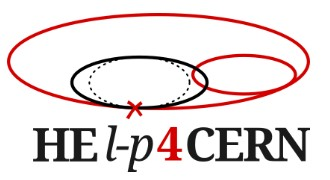
\includegraphics[width=1.8cm]{HELP4CERN.jpg}};
	\end{tikzpicture}
\end{frame}





% --------------------------------------------------------------------------
% Slide 15
% --------------------------------------------------------------------------
\begin{frame}{Flagship $\gamma\gamma$ channels III: $ZZ$, $t\bar t$, and heavy exclusive final states}
	\begin{itemize}
		\justifying
		\item Loop-induced $\gamma\gamma\to ZZ$ is especially interesting because it is absent at tree level in the Standard Model and therefore provides a clean probe of high-mass electroweak dynamics.
		\item Representative elastic cross sections at 3.7 TeV are:
		\begin{itemize}
			\justifying
			\item $\sigma_{\mathrm{el}}(\gamma\gamma\to ZZ)\simeq 0.284$ fb,
			\item $\sigma_{\mathrm{el}}(\gamma\gamma\to t\bar t)\simeq 0.486$ fb.
		\end{itemize}
		\justifying
		\item Although smaller than the $\tau\tau$ and $WW$ cases, these channels gain importance because they probe loop structure, heavy thresholds, and the onset of high-energy electroweak / top dynamics.
		\item The same photon-induced framework also extends to exclusive pair production of BSM charged states such as higgsinos and sleptons.
	\end{itemize}
	
	%\placeholdergraphic{Suggested screenshot source:\\
		%From \texttt{Hamzeh\_Khanpour\_CERN\_9Dec.pdf}, slides 7--9 (ZZ, $t\bar t$, and SUSY-pair plots).}{0.25\textheight}
	
	\begin{tikzpicture}[remember picture,overlay]
		\node[anchor=north east, xshift=-0.10cm, yshift=-1.25cm]
		at (current page.north east)
		{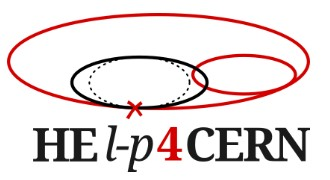
\includegraphics[width=1.8cm]{HELP4CERN.jpg}};
	\end{tikzpicture}
\end{frame}









\begin{frame}
	
	
	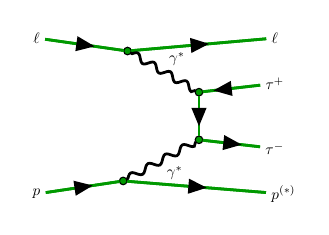
\begin{tikzpicture}[scale=0.55, transform shape]
		\begin{feynman}
			
			%------------------------------------------------
			% External states
			%------------------------------------------------
			\vertex (i1) at (-2.8,  1.8) {\(\ell\)};
			\vertex (i2) at (-2.8, -1.8) {\(p\)};
			
			\vertex (o1) at ( 2.7,  1.8) {\(\ell\)};
			\vertex (o2) at ( 2.9, -1.8) {\(p^{(*)}\)};
			
			\vertex (t1) at ( 2.7,  0.75) {\(\tau^{+}\)};
			\vertex (t2) at ( 2.7, -0.75) {\(\tau^{-}\)};
			
			%------------------------------------------------
			% Interaction vertices
			%------------------------------------------------
			\vertex [dot, fill=green!60!black, minimum size=5pt] (v1) at (-0.7,  1.5) {};
			\vertex [dot, fill=green!60!black, minimum size=5pt] (v2) at (-0.8, -1.5) {};
			
			\vertex [dot, fill=green!60!black, minimum size=5pt] (v3) at ( 0.95,  0.55) {};
			\vertex [dot, fill=green!60!black, minimum size=5pt] (v4) at ( 0.95, -0.55) {};
			
			%------------------------------------------------
			% Diagram
			%------------------------------------------------
			\diagram*{
				(i1) -- [fermion, draw=green!60!black, line width=1.0pt] (v1)
				-- [fermion, draw=green!60!black, line width=1.0pt] (o1),
				
				(i2) -- [fermion, draw=green!60!black, line width=1.0pt] (v2)
				-- [fermion, draw=green!60!black, line width=1.0pt] (o2),
				
				(v1) -- [photon, edge label=\(\gamma^\ast\), line width=1.0pt] (v3),
				(v2) -- [photon, edge label'=\(\gamma^\ast\), line width=1.0pt] (v4),
				
				(v3) -- [fermion, draw=green!60!black, line width=1.0pt] (v4),
				
				(v3) -- [anti fermion, draw=green!60!black, line width=1.0pt] (t1),
				(v4) -- [fermion, draw=green!60!black, line width=1.0pt] (t2),
			};
			
		\end{feynman}
	\end{tikzpicture}
	
	
\end{frame}







%=====================================================
\begin{frame}{Representative Higgs-production channels at LH$\mu$C}
	
	\begin{columns}%[T,onlytextwidth]
		
		%------------------------------------------------
		\begin{column}{0.48\textwidth}
			\centering
			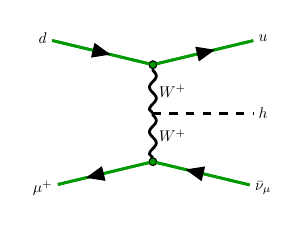
\begin{tikzpicture}[scale=0.56, transform shape]
				\begin{feynman}
					\vertex (i1) at (-2.5,  1.7) {\(d\)};
					\vertex (i2) at (-2.5, -1.7) {\(\mu^{+}\)};
					\vertex [dot, fill=green!60!black, minimum size=5pt] (v1) at (0,1.1) {};
					\vertex [dot, fill=green!60!black, minimum size=5pt] (v2) at (0,-1.1) {};
					\vertex (o1) at (2.5,  1.7) {\(u\)};
					\vertex (o2) at (2.5, -1.7) {\(\bar{\nu}_{\mu}\)};
					\vertex (h1) at (2.5,0.0) {\(h\)};
					\vertex (m1) at (0,0.0);
					
					\diagram*{
						(i1) -- [fermion, draw=green!60!black, line width=1.0pt] (v1)
						-- [fermion, draw=green!60!black, line width=1.0pt] (o1),
						(i2) -- [anti fermion, draw=green!60!black, line width=1.0pt] (v2)
						-- [anti fermion, draw=green!60!black, line width=1.0pt] (o2),
						(v1) -- [boson, edge label=\(W^{+}\), line width=1.0pt] (m1),
						(m1) -- [boson, edge label=\(W^{+}\), line width=1.0pt] (v2),
						(m1) -- [scalar, line width=1.0pt] (h1),
					};
				\end{feynman}
				\node[blue!90!black, font=\scriptsize] at (0.0,0.82) {\textbf{}};
				\node[blue!90!black, font=\scriptsize] at (0.0,-0.82) {\textbf{}};
			\end{tikzpicture}
			
			\vspace{0.2em}
			{\scriptsize CC contribution to \(\mu^{+} d \to \bar{\nu}_{\mu}\,u\,h\)}
		\end{column}
		
		%------------------------------------------------
		\begin{column}{0.48\textwidth}
			\centering
			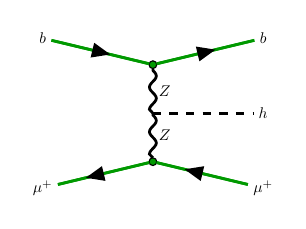
\begin{tikzpicture}[scale=0.56, transform shape]
				\begin{feynman}
					\vertex (i1) at (-2.5,  1.7) {\(b\)};
					\vertex (i2) at (-2.5, -1.7) {\(\mu^{+}\)};
					\vertex [dot, fill=green!60!black, minimum size=5pt] (v1) at (0,1.1) {};
					\vertex [dot, fill=green!60!black, minimum size=5pt] (v2) at (0,-1.1) {};
					\vertex (o1) at (2.5,  1.7) {\(b\)};
					\vertex (o2) at (2.5, -1.7) {\(\mu^{+}\)};
					\vertex (h1) at (2.5,0.0) {\(h\)};
					\vertex (m1) at (0,0.0);
					
					\diagram*{
						(i1) -- [fermion, draw=green!60!black, line width=1.0pt] (v1)
						-- [fermion, draw=green!60!black, line width=1.0pt] (o1),
						(i2) -- [anti fermion, draw=green!60!black, line width=1.0pt] (v2)
						-- [anti fermion, draw=green!60!black, line width=1.0pt] (o2),
						(v1) -- [boson, edge label=\(Z\), line width=1.0pt] (m1),
						(m1) -- [boson, edge label=\(Z\), line width=1.0pt] (v2),
						(m1) -- [scalar, line width=1.0pt] (h1),
					};
				\end{feynman}
				\node[blue!90!black, font=\scriptsize] at (0.0, 0.82) {\textbf{}};
				\node[blue!90!black, font=\scriptsize] at (0.0,-0.82) {\textbf{}};
			\end{tikzpicture}
			
			\vspace{0.2em}
			{\scriptsize NC contribution to \(\mu^{+} b \to \mu^{+}\,b\,h\)}
		\end{column}
		
	\end{columns}
	
\end{frame}
%=====================================================






% --------------------------------------------------------------------------
% Slide 8
% --------------------------------------------------------------------------
\begin{frame}{Precision Higgs case study: $h\to b\bar b$ and coupling prospects}
	\begin{columns}[T]
		
		\begin{column}{0.58\textwidth}
			\begin{itemize}
				\justifying
				\item A concrete benchmark already exists for the charged-current VBF process with $h\to b\bar b$.
				
				\item The parton showering, fast detector simulation, and a cut-based analysis were used to estimate:
				\begin{itemize}
					\justifying
					\item $\Delta \sigma/\sigma \simeq 1.19\%$ and $0.69\%$ for the two $\mu p$ collider setups,
					\item corresponding benchmark sensitivities of about $0.77\%$ and $0.60\%$ on $g_{hbb}$.
				\end{itemize}
				\justifying
				\item This strongly supports the claim that \LHCmu{} can be a competitive Higgs factory.		
				%\item \textbf{Important caveat:} the global coupling-fit programme is still under development, and naive recycling of LHeC signal-strength projections is not yet sufficient for the final LH$\mu$C coupling case.
			\end{itemize}
		\end{column}
		
		\begin{column}{0.40\textwidth}
			\begin{table}
				\centering
				\scriptsize
				\renewcommand{\arraystretch}{1.15}
				\setlength{\tabcolsep}{3.5pt}
				\begin{tabular}{lcc}
					\toprule
					& $\mu p$-1 & $\mu p$-2 \\
					\midrule
					$\sigma_{\rm sig}$ [pb] & 0.24 & 0.39 \\
					$\sigma_{\rm bgd\text{-}Z}$ [pb] & 0.30 & 0.50 \\
					$\sigma_{\rm bgd\text{-}mj}$ [pb] & 357.9 & 563.8 \\
					$\epsilon^{\rm sig}_{\rm cut}$ & 0.22 & 0.21 \\
					$\epsilon^{\rm bgd\text{-}Z}_{\rm cut}$ & 0.025 & 0.025 \\
					$\epsilon^{\rm bgd\text{-}mj}_{\rm cut}$ & $9.7\times10^{-5}$ & $1.23\times10^{-4}$ \\
					\midrule
					$\Delta \sigma/\sigma$ & 1.19\% & 0.69\% \\
					$\Delta g_{hbb}/g_{hbb}$ & 0.77\% & 0.60\% \\
					\bottomrule
				\end{tabular}
				\caption{\justifying \scriptsize Benchmark $h\to b\bar b$ case study at $\mu p$ colliders: signal and background cross sections, cut efficiencies, and projected sensitivities for the Higgs coupling to bottom quarks.}
			\end{table}
		\end{column}
	\end{columns}
	\begin{tikzpicture}[remember picture,overlay]
		\node[anchor=north east, xshift=-0.10cm, yshift=-1.25cm]
		at (current page.north east)
		{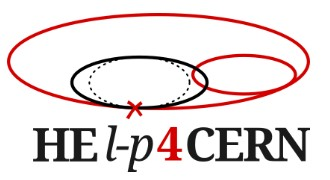
\includegraphics[width=1.5cm]{HELP4CERN.jpg}};
	\end{tikzpicture}
\end{frame}





\begin{frame}{Electroweak programme and EFT opportunities}
	\begin{itemize} 
		\justifying 
		\small 
		
		\item Beyond Higgs rates, LH$\mu$C offers a broader electroweak programme based on high-$Q^2$ DIS, vector-boson fusion, and photon-induced reactions.  
		
		\item The larger kinematic span relative to the LHeC is expected to strengthen sensitivity to key electroweak observables, in particular $m_W$ and $\sin^2\theta_W$, while also extending the SMEFT lever arm.  
		
		\item Particularly interesting electroweak opportunities include:
		\begin{itemize}
			\justifying 
			\small 
			\item high-scale measurements of the weak mixing angle and its running, 
			\item precision access to light-quark weak neutral-current couplings through $\gamma Z$ interference and $Z$ exchange,
			\item improved sensitivity to $m_W$ in a clean DIS environment,
			\item electroweak/top measurements linked to the $Wtb$ vertex and direct sensitivity to $V_{ts}$,
			\item SMEFT directions complementary to those probed at $pp$ and $e^+e^-$ machines,
			\item and photon-induced electroweak EFT sensitivity in $\gamma\gamma\to W^+W^-$, $ZZ$, and heavy final states.
		\end{itemize}
		
		\item Overall, LH$\mu$C is expected to extend the precision electroweak reach beyond that projected for the LHeC.  
	\end{itemize}
	
	\begin{tikzpicture}[remember picture,overlay]
		\node[anchor=north east, xshift=-0.10cm, yshift=-1.25cm]
		at (current page.north east)
		{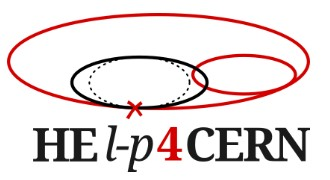
\includegraphics[width=1.5cm]{HELP4CERN.jpg}};
	\end{tikzpicture}
\end{frame}








% --------------------------------------------------------------------------
% Slide 14
% --------------------------------------------------------------------------
\begin{frame}{\LHCmu{} as a top factory}
	\begin{columns}[T]
		\begin{column}{0.99\textwidth}
			\begin{itemize}
				\justifying
				\item The most striking HET advantage of \LHCmu{} relative to the LHeC is the \textbf{top sector}.
				\item Inclusive benchmark rates:
				\begin{itemize}
					\item single top: $21.26$ pb at 500 GeV and $36.77$ pb at 1 TeV,
					\item $t\bar t$: $1.03$ pb at 500 GeV and $2.23$ pb at 1 TeV.
				\end{itemize}
				\justifying
				\item For the benchmark integrated luminosities, this translates into:
				\begin{itemize}
					\justifying
					\item $\sim 5.3\times10^6$ single-top events at 500 GeV,
					\item $\sim 2.6\times10^5$ $t\bar t$ events at 500 GeV,
					\item $\sim 3.7\times10^7$ single-top events at 1 TeV,
					\item $\sim 2.2\times10^6$ $t\bar t$ events at 1 TeV.
				\end{itemize}
				\justifying
				\item This is why the current collaboration narrative repeatedly describes \LHCmu{} as a genuine top factory.
			\end{itemize}
		\end{column}
		%\begin{column}{0.38\textwidth}
		%\placeholdergraphic{Best compact figure source: \texttt{Hamzeh\_Khanpour\_Help4CERN\_13Jan.pdf}, slide with inclusive top and Higgs cross-section table; \\
			%Alternative: \texttt{LHuC\_KP.pdf}, page 19.}{0.60\textheight}
		%\end{column}
	\end{columns}
	\begin{tikzpicture}[remember picture,overlay]
		\node[anchor=north east, xshift=-0.10cm, yshift=-1.25cm]
		at (current page.north east)
		{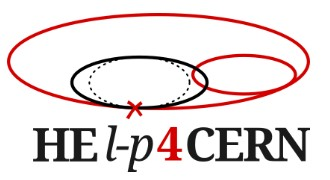
\includegraphics[width=1.8cm]{HELP4CERN.jpg}};
	\end{tikzpicture}
\end{frame}






% --------------------------------------------------------------------------
% Slide 15
% --------------------------------------------------------------------------
\begin{frame}{Top event topology, acceptance, and why \LHCmu{} helps experimentally}
	\begin{columns}[T]
		\begin{column}{0.99\textwidth}
			\begin{itemize}
				\justifying
				\item Beyond inclusive rates, dedicated semileptonic $t\bar t$ studies indicate that the \LHCmu{} event topology is more central than the LHeC one.
				\item This matters because the gain at generator level is not purely from larger cross sections; it is also supported by strong kinematic acceptance.
				\item Representative semileptonic acceptance numbers show only modest degradation even for tighter lepton rapidity cuts, with the \LHCmu{} case remaining particularly favourable.
				\item Therefore the larger top rates are not merely formal parton-level advantages: they are likely to remain exploitable after realistic selections.
			\end{itemize}
		\end{column}
		%\begin{column}{0.38\textwidth}
		%\placeholdergraphic{From \texttt{Hamzeh\_Khanpour\_CERN\_29Dec.pdf}, slides 10--13: acceptance table, light-jet pseudorapidity, reconstructed $W$ mass, and lepton-$\eta$ comparison.}{0.60\textheight}
		%\end{column}
	\end{columns}
	%\takehome{For the talk, one acceptance/centrality slide is enough; do not overload with many detector-level details.}
	\begin{tikzpicture}[remember picture,overlay]
		\node[anchor=north east, xshift=-0.10cm, yshift=-1.25cm]
		at (current page.north east)
		{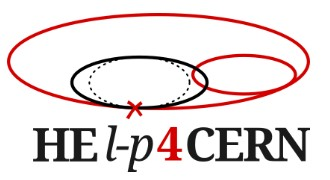
\includegraphics[width=1.8cm]{HELP4CERN.jpg}};
	\end{tikzpicture}
\end{frame}







% --------------------------------------------------------------------------
% Slide 15 
% --------------------------------------------------------------------------
\begin{frame}{Rare top, FCNC, and EFT directions}
	\begin{itemize}
		\justifying
		\item The top sector at \LHCmu{} is interesting not only for statistics, but also for \textbf{rare processes and anomalous couplings}.
		\item Dedicated studies already show that top-FCNC sensitivities improve substantially from the LHeC to the \LHCmu{}, reflecting both the higher rates and the harder kinematics.
		\item The characteristic $\mu p$ topology provides a useful environment for studying anomalous $tq\gamma$, $tqZ$, and $tqH$ interactions, as well as broader EFT deformations in single-top and associated channels.
		%\item In the presentation, this part should be framed as one representative example of how the enormous top samples can be converted into BSM reach.
	\end{itemize}
	
	%\placeholdergraphic{Suggested source: \texttt{Hamzeh\_Khanpour\_Help4CERN\_3Feb.pdf}, slides 14--18 for FCNC cross-section/coupling dependence and kinematic distributions.}{0.28\textheight}
	\begin{tikzpicture}[remember picture,overlay]
		\node[anchor=north east, xshift=-0.10cm, yshift=-1.25cm]
		at (current page.north east)
		{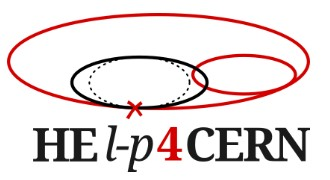
\includegraphics[width=1.8cm]{HELP4CERN.jpg}};
	\end{tikzpicture}
\end{frame}







% --------------------------------------------------------------------------
% Slide 17
% --------------------------------------------------------------------------
\begin{frame}{Representative BSM benchmarks: RPV SUSY and color-octet muons}
	\begin{columns}[T]
		\begin{column}{0.99\textwidth}
			\begin{itemize}
				\justifying
				\item \textbf{RPV SUSY:} The $\mu p$ collisions can probe resonantly produced squarks with coupling reaches stronger than HL-LHC bounds in the on-shell regime.
				\item \textbf{Color-octet muons:} A 5$\sigma$ discovery reach of about:
				\begin{itemize}
					\justifying
					\item $\sim 2.3$ TeV at the HL-LHC,
					\item $\sim 3.0$ TeV for the 500 GeV \LHCmu{} option,
					\item $\sim 4.2$ TeV for the 1 TeV \LHCmu{} option.
				\end{itemize}
				\justifying
				\item These examples are sufficient to demonstrate that the BSM case is not generic hype: it is tied to concrete channels where the $\mu p$ initial state is a genuine advantage.
			\end{itemize}
		\end{column}
		%\begin{column}{0.40\textwidth}
		%\placeholdergraphic{Suggested screenshot source:\\
			%RPV: \texttt{Physics potential of a muon-proton collider.pdf}, Fig.~2 / page 4 \\
			%OR \texttt{HELP4CERN.pdf}, Fig.~2 / pages 13--15.\\[0.8ex]
			%Color-octet muon: \texttt{HELP4CERN.pdf}, Fig.~4 / pages 15--17.}{0.60\textheight}
		%\end{column}
	\end{columns}
	\begin{tikzpicture}[remember picture,overlay]
		\node[anchor=north east, xshift=-0.10cm, yshift=-1.25cm]
		at (current page.north east)
		{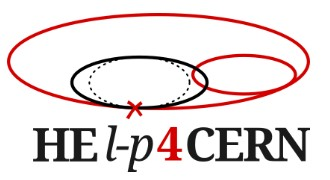
\includegraphics[width=1.8cm]{HELP4CERN.jpg}};
	\end{tikzpicture}
	\vspace{0.3em}
	{\justifying \scriptsize
		\setlength{\fboxsep}{4pt}%
		\colorbox{green!15}{%
			\parbox{0.92\linewidth}{%
				Kingman Cheung and Zeren Simon Wang, \textit{Physics potential of a muon-proton collider}, Phys.\ Rev.\ D~103 (2021) 116009.%
			}%
		}%
	}
\end{frame}






